% !TEX program = pdflatex
% !TEX root = ESM_1.tex
% Supplementary material for manuscript.tex.
% Overleaf/latexmk: latexmkrc updates both documents' external references.
% Local build: powershell -File compile.ps1
% Auxiliary results and method details accompany the core proofs in the main appendix.
\documentclass[11pt,a4paper,leqno]{article}

\usepackage[T1]{fontenc}
\usepackage{iftex}
\ifPDFTeX
  \usepackage[utf8]{inputenc}
\fi
\usepackage[left=27mm,right=27mm,top=25mm,bottom=25mm,headheight=14pt]{geometry}
\usepackage{amsmath,amssymb,amsthm,mathtools}
\usepackage{newtxtext,newtxmath}
\usepackage{microtype}
\usepackage{graphicx}
\usepackage{placeins}
% Keep float groups compact instead of spreading them over a whole page.
\makeatletter
\setlength{\@fptop}{0pt}
\setlength{\@fpsep}{12pt}
\setlength{\@fpbot}{0pt plus1fil}
\makeatother
\setcounter{topnumber}{5}
\setcounter{totalnumber}{6}
\renewcommand{\topfraction}{0.9}
\renewcommand{\textfraction}{0.08}
\renewcommand{\floatpagefraction}{0.85}
\setlength{\floatsep}{10pt plus2pt minus2pt}
\setlength{\textfloatsep}{10pt plus2pt minus2pt}
\setlength{\intextsep}{10pt plus2pt minus2pt}
\graphicspath{{figures/}}
\usepackage{booktabs,array}
\usepackage[authoryear]{natbib}
\setcitestyle{aysep={}}
% The Springer bibliography style also supports this standalone supplement.
\providecommand{\bibcommenthead}{}
\usepackage{xcolor}
\definecolor{suppblue}{RGB}{0,65,120}

% Import main-text labels only; the supplement keeps its own bibliography.
% Main-document reference syntax: \ref{main-thm:fixed_generator},
% \eqref{main-eq:ls_clt}. Moved labels retain their names; new supplement labels use supp:.
% latexmkrc generates the main document's labels automatically.
\usepackage{xr-hyper}
\usepackage[colorlinks=true,linkcolor=suppblue,citecolor=suppblue,urlcolor=suppblue]{hyperref}
\usepackage{xurl}
\providecommand{\burl}[1]{\url{#1}}
% Keep remote-link page state local with the XeTeX driver in TeX Live 2022.
\ifXeTeX
  \AddToHook{cmd/hyper@linkfile/before}{\begingroup}
  \AddToHook{cmd/hyper@linkfile/after}{\endgroup}
\fi
\externaldocument[main-][nocite]{manuscript}[manuscript.pdf]

\usepackage{titlesec}
\titleformat{\section}
  {\normalfont\large\centering\scshape}
  {Supplementary Appendix \thesection:}{0.6em}{}
\titleformat{\subsection}
  {\normalfont\normalsize\bfseries}
  {\thesubsection}{0.6em}{}
\titlespacing*{\section}{0pt}{2ex plus 0.5ex minus 0.2ex}{1ex}
\titlespacing*{\subsection}{0pt}{1.6ex plus 0.4ex}{0.7ex}

\usepackage{fancyhdr}
\pagestyle{fancy}
\fancyhf{}
\fancyhead[L]{\small\textsc{Supplementary Material}}
\fancyhead[R]{\small Optimal Subsampling}
\fancyfoot[C]{\thepage}
\renewcommand{\headrulewidth}{0pt}
\fancypagestyle{plain}{%
  \fancyhf{}
  \fancyfoot[C]{\thepage}
  \renewcommand{\headrulewidth}{0pt}
}

% Independent numbering: (A.1), Lemma A.1, Table B.1, and so on.
\numberwithin{equation}{section}
\numberwithin{figure}{section}
\numberwithin{table}{section}
\theoremstyle{plain}
\newtheorem{lemma}{Lemma}[section]
\newtheorem{theorem}[lemma]{Theorem}
\newtheorem{proposition}[lemma]{Proposition}
\newtheorem{corollary}[lemma]{Corollary}
\theoremstyle{definition}
\newtheorem{definition}[lemma]{Definition}
\newtheorem{assumption}[lemma]{Assumption}
\newtheorem{example}[lemma]{Example}
\theoremstyle{remark}
\newtheorem{remark}[lemma]{Remark}
\renewcommand{\proofname}{\normalfont\scshape Proof}
\allowdisplaybreaks[2]
\setlength{\parindent}{1.3em}
\setlength{\parskip}{0pt}
% Keep single paragraph lines from being stranded at page boundaries.
\clubpenalty=10000
\widowpenalty=10000
\setlength{\emergencystretch}{1em}
\AtBeginDocument{%
  \setlength{\abovedisplayskip}{8pt plus2pt minus2pt}%
  \setlength{\belowdisplayskip}{8pt plus2pt minus2pt}%
  \setlength{\abovedisplayshortskip}{0pt plus2pt}%
  \setlength{\belowdisplayshortskip}{4pt plus2pt minus1pt}%
}

% Mathematical commands agree with the current main manuscript.
\newcommand{\bx}{\mathbf{x}}
\newcommand{\bX}{\mathbf{X}}
\newcommand{\bY}{\mathbf{Y}}
\newcommand{\bbeta}{\boldsymbol{\beta}}
\newcommand{\bSigma}{\boldsymbol{\Sigma}}
\newcommand{\cO}{\mathcal{O}}
\newcommand{\RR}{\mathbb{R}}
\newcommand{\EE}{\mathbb{E}}
\newcommand{\Var}{\mathrm{Var}}
\newcommand{\tr}{\mathrm{tr}}
\newcommand{\R}{\mathbb R}
\newcommand{\E}{\mathbb E}
\newcommand{\Prob}{\mathbb P}
\newcommand{\norm}[1]{\lVert#1\rVert}
\newcommand{\heading}[1]{\medskip\noindent\textbf{#1}\enspace}

\hypersetup{
  pdftitle={Supplementary Material: Optimal Subsampling for Regularized Linear Regression: A Generator-Function Framework},
  pdfauthor={Junchen Li, Ying-Ao Wang, Ye Zhang}
}

\begin{document}
\thispagestyle{plain}

% Title and author names mirror the current main manuscript.
\begin{center}
  {\normalsize\textbf{Online Resource 1}\par}
  \vspace{0.3em}
  {\large\bfseries SUPPLEMENTARY MATERIAL TO\\[0.4em]
  ``Optimal Subsampling for Regularized Linear Regression:\\
  A Generator-Function Framework''\par}
  \vspace{0.3em}
  {\normalsize Journal: \emph{Statistics and Computing}\par}
  \vspace{0.5em}
  {\normalsize\textsc{Junchen Li}\textsuperscript{1},
  \textsc{Ying-Ao Wang}\textsuperscript{1} and
  \textsc{Ye Zhang}\textsuperscript{2}\par}
  \vspace{0.3em}
  {\small
  \textsuperscript{1}School of Mathematics and Statistics,\\
  Beijing Institute of Technology, Beijing 100081, China\par
  \vspace{0.3em}
  \textsuperscript{2}MSU-BIT-SMBU Joint Research Center for Applied Mathematics,\\
  Shenzhen MSU-BIT University, Shenzhen 518172, China\par
  \vspace{0.3em}
  E-mail addresses:\\
  Junchen Li: \href{mailto:lijunchen@bit.edu.cn}{\nolinkurl{lijunchen@bit.edu.cn}};\quad
  Ying-Ao Wang: \href{mailto:wya@bit.edu.cn}{\nolinkurl{wya@bit.edu.cn}}\\
  Ye Zhang: \href{mailto:ye.zhang@smbu.edu.cn}{\nolinkurl{ye.zhang@smbu.edu.cn}}\par}
  % Corresponding-author identity remains unconfirmed in the main manuscript.
  % All established author contacts are listed without inferring a designation.
\end{center}

This document accompanies the main article. Notation and assumptions follow
the main article unless stated otherwise. Equations, figures, tables, and
auxiliary results in this supplement have independent appendix numbering.
The main article contains the theorem statements; its
Appendix~\ref{main-app:core-proofs} contains the complete core proofs.
Here we give auxiliary lemmas, the remaining proofs, and detailed
verification of the accelerated and inertial generators.

\appendix
\section{Auxiliary lemmas}
\label{supp:sec:lemmas}
We use the notation and assumptions of Sections~\ref{main-subsec:fixed_generator_theory}
and~\ref{main-subsec:growing_column_arrays} of the main article.

\subsection{Local matrix expansions and finite-atom sampling}
The first-order divided-difference formula below is the classical
Fr\'echet derivative of a matrix function; see \citet[Chapter~3]{higham2008functions}.
We include a proof under the local assumptions used here.
\begin{lemma}[Local matrix expansion]\label{lem:local_matrix}
Under (A1), for symmetric perturbations $E$ supported on $\mathcal R_M$,
\[
 g(M+E)-g(M)=Dg_M[E]+o(\|E\|_2).
\]
Here the assertion concerns sufficiently small $E$, and zero blocks cancel.
If $U$ is an orthonormal eigenbasis of $\mathcal R_M$ with positive
eigenvalues $\lambda_1,\ldots,\lambda_\rho$, where $\rho=\dim\mathcal R_M$, then
\[
 \begin{aligned}
 Dg_M[E]&=U\{\mathcal L_g\circ(U^\top EU)\}U^\top,\\
 (\mathcal L_g)_{ab}&=
 \begin{cases}
 [g(\lambda_a)-g(\lambda_b)]/(\lambda_a-\lambda_b),
       &\lambda_a\ne\lambda_b,\\
 g'(\lambda_a),&\lambda_a=\lambda_b.
 \end{cases}
 \end{aligned}
\]
Under (A2), the remainder is bounded by $C\|E\|_2^2$ for $\|E\|_2\le\delta$,
after decreasing the locally admissible radius if necessary.
\end{lemma}
\begin{proof}
Work first on $\mathcal R_M$, where $M$ is positive definite.
Let $P$ be the Hermite interpolation polynomial matching $g$ and $g'$
at every distinct eigenvalue of $M$. For $t$ near such an eigenvalue $\mu$,
$(g-P)(t)=o(|t-\mu|)$ under (A1), and is $O(|t-\mu|^2)$ under (A2).
Weyl's eigenvalue bound places each eigenvalue of $M+E$ within $\|E\|_2$
of an eigenvalue of $M$. Spectral calculus consequently gives
$\|(g-P)(M+E)\|_2=o(\|E\|_2)$, respectively $O(\|E\|_2^2)$.
Since $(g-P)(M)=0$, expansion of the fixed polynomial $P$ proves the claim.
Its derivative has the displayed divided differences because $P$ matches
both values and first derivatives of $g$. Repeated eigenvalues therefore
cause no ambiguity. Extending by zero gives the asserted effective-space
derivative; the common value $g(0)$ cancels on $\mathcal R_M^\perp$.
\end{proof}

\begin{lemma}[Finite-atom bounds]\label{lem:finite_atoms}
Let $z_1,\ldots,z_{N_0}$ and $b_1,\ldots,b_{N_0}$ be fixed finite vectors,
$\varpi_i>0$, $\sum_i\varpi_i=1$, and let $K_t$ be i.i.d.\ with this law.
Set
\[
 M=\sum_i z_i z_i^\top,\quad
 \widehat M=\frac1N\sum_t\frac{z_{K_t}z_{K_t}^\top}{\varpi_{K_t}},
 \quad d=\sum_i b_i,\quad
 \widehat d=\frac1N\sum_t\frac{b_{K_t}}{\varpi_{K_t}}.
\]
For $q=2,4$,
\[
 \E\|\widehat M-M\|_2^q+\E\|\widehat d-d\|_2^q=O(N^{-q/2}).
\]
For every fixed $\delta>0$ there are constants $C,c>0$ such that
$\Prob(\|\widehat M-M\|_2>\delta)\le Ce^{-cN}$.
Both spectra lie in $[0,B]$, where $B=\max_i\|z_i\|_2^2/\varpi_i$,
and $\widehat d$ is uniformly bounded over all sample realizations.
If some $z_i\ne0$, there is $\kappa>0$, independent of $N$, such that
every nonzero sampled matrix satisfies
$\lambda_{\min}^+(\widehat M)\ge\kappa/N$.
\end{lemma}
\begin{proof}
Every centered coordinate of either empirical average is an average of
bounded, independent, mean-zero variables. Its second moment is $O(N^{-1})$;
expanding its fourth moment leaves only paired or identical indices and
gives $O(N^{-2})$. Equivalence of norms in the fixed-dimensional spaces
proves the moment bounds. Applying the scalar bounds of
\citet{hoeffding1963probability} to the finitely
many matrix coordinates and taking a union bound proves the exponential bound.
The spectral upper bound follows because $\widehat M$ and $M$ are convex
combinations of $z_i z_i^\top/\varpi_i$; the bound for $\widehat d$ is similar.
For each nonempty subset $T$ of the nonzero atoms, put
$M_T=\sum_{i\in T}z_i z_i^\top/\varpi_i$ and set
$\kappa=\min_T\lambda_{\min}^+(M_T)>0$.
There are finitely many such subsets. If $T$ is the set of sampled nonzero
atoms, $\widehat M$ and $M_T$ have the same range and
$\widehat M\succeq M_T/N$ on that range. This proves the lower bound.
If no nonzero atom is sampled, $\widehat M=0$ and the last assertion is vacuous.
\end{proof}

\subsection{A dimension-free matrix remainder}
\label{supp:matrix-curvature}
\begin{lemma}[A dimension-free local matrix remainder]
\label{lem:matrix_curvature}
Let \(M,E\) be real symmetric matrices and let \(f\) be twice continuously
differentiable on an open interval containing a compact interval \(I\).
If the spectrum of \(M+tE\) belongs to \(I\) for every \(0\le t\le1\),
then
\[
 \|f(M+E)-f(M)-Df_M[E]\|_2
 \le \frac12\sup_{u\in I}|f''(u)|\,\|E\|_F^2.
\]
\end{lemma}
\begin{proof}
Set \(b=\sup_I|f''|\). For a matrix \(A\) on the path, the
second-derivative formula for \(C^2\) scalar functions along symmetric matrix paths
\citep[Theorems~6--7]{bickel2013differentiating} gives, in its eigenbasis,
\[
 (D^2f_A[E,E])_{ik}
 =2\sum_j f^{[2]}(\lambda_i,\lambda_j,\lambda_k)E_{ij}E_{jk}.
\]
The Genocchi--Hermite integral representation of the second divided difference,
including repeated nodes \citep[Eq.~(52)]{deboor2005divided}, gives
\(|f^{[2]}|\le b/2\). If \(F\) is the entrywise
absolute value of \(E\) in this basis, then
\(|D^2f_A[E,E]_{ik}|\le b(F^2)_{ik}\), where \(F^2\) is a matrix product.
Entrywise nonnegative domination therefore yields
\(\|D^2f_A[E,E]\|_2\le b\|F^2\|_2
 \le b\|F\|_F^2=b\|E\|_F^2\).
Orthogonal changes of basis preserve the latter norm.
Integrating \(D^2f_{M+tE}[E,E]\) with weight \(1-t\) proves the assertion.
\end{proof}

If \(f_N\in C^2\) on an open neighborhood of
\([m_N-\delta_N,M_N+\delta_N]\), Lemma~\ref{lem:matrix_curvature}
verifies \eqref{main-eq:array_local_taylor} with
\[
 K_N=\tfrac12\sup_{u\in[m_N-\delta_N,M_N+\delta_N]}|f_N''(u)|.
\]
The derivative and this bound concern the effective space only.
For example, the Moore--Penrose inverse need not be differentiable in
directions that change rank. A neighborhood without a specified radius
does not by itself verify \eqref{main-eq:array_generator_rates}.

\subsection{Sampling identities}\label{sec:sampling_identities}
\begin{lemma}[Unbiased Gram and cross-moment estimates]
\label{lem:sampling_weight_unbiasedness}
For the stated importance sampling schemes,
\[
 \E\widehat H_N=H,\qquad \E\widehat A_N=A,\qquad
 \E\widehat c_N=c.
\]
If every coordinate is retained with positive probability,
$\E(SS^\top)=I_p$ and $\E W_{\rm row}=I_n$.
If zero atoms are omitted, these last identities use the corresponding
coordinate projections instead; the three Gram and cross-moment identities
remain unchanged.
\end{lemma}
\begin{proof}
For example,
$\E[a_{J}a_{J}^\top/\pi_J]=\sum_j a_ja_j^\top=H$ and
$\E[x_Iy_I/\nu_I]=\sum_i x_iy_i=c$.
Linearity of expectation proves the assertions; omitted zero atoms
contribute zero to the relevant sums.
\end{proof}

\begin{lemma}[Centered residual score covariance]
\label{lem:row_residual_score_variance}
For a fixed residual vector $\eta$ and fixed row probabilities,
\[
 \operatorname{Cov}(X^\top W_{\rm row}\eta)
 =\frac1N\left\{\sum_i\frac{\eta_i^2}{\nu_i}x_ix_i^\top
                 -(X^\top\eta)(X^\top\eta)^\top\right\}.
\]
\end{lemma}
\begin{proof}
The one-draw score is $x_I\eta_I/\nu_I$, with mean $X^\top\eta$
and second moment $\sum_i\eta_i^2x_ix_i^\top/\nu_i$.
Independence and averaging give the result. The centering term vanishes
for full-data LS residuals, but generally not for regularized residuals.
\end{proof}

\subsection{Spectral representations and classical generators}
\label{supp:sec:classical_generators}
This subsection records the spectral and normalization details used in
Section~\ref{main-sec:formulation} of the main article.

Consider the singular value decomposition (SVD) of the design matrix
$X_n\in\RR^{n\times p}$:
\begin{equation*}
    X_n=U\Lambda V^\top,
\end{equation*}
where $U\in\RR^{n\times n}$ and $V\in\RR^{p\times p}$ are orthogonal,
and $\Lambda\in\RR^{n\times p}$ is rectangular diagonal. Its nonzero
diagonal entries are $\sqrt{\lambda_1},\ldots,\sqrt{\lambda_\rho}$,
where $\rho=\operatorname{rank}(X_n)$ and
$\lambda_1\ge\cdots\ge\lambda_\rho>0$. Thus
$\lambda_j=\sigma_j^2(X_n)$, and direct multiplication gives
\[
    \begin{aligned}
    X_n^\top X_n&=V(\Lambda^\top\Lambda)V^\top,\\
    X_nX_n^\top&=U(\Lambda\Lambda^\top)U^\top.
    \end{aligned}
\]
Using the same singular system, define
\begin{equation*}
\begin{aligned}
    g_\alpha(X_n^\top X_n)
        &:=Vg_\alpha(\Lambda^\top\Lambda)V^\top,\\
    g_\alpha(X_nX_n^\top)
        &:=Ug_\alpha(\Lambda\Lambda^\top)U^\top,
\end{aligned}
\end{equation*}
where $g_\alpha$ is applied separately to each diagonal entry of the
diagonal matrices. In particular, when $X_n$ has full column rank,
\[
    g_\alpha(X_n^\top X_n)
    =V\operatorname{diag}\bigl(g_\alpha(\lambda_1),\ldots,
                              g_\alpha(\lambda_p)\bigr)V^\top.
\]
In the column-sampling regime $p>n$ with full row rank, $\rho=n$ and
$\Lambda=[\operatorname{diag}(\sqrt{\lambda_1},\ldots,
\sqrt{\lambda_n})\ \ 0]$. Hence the corresponding dual definition is
\[
    g_\alpha(X_nX_n^\top)
    =U\operatorname{diag}\bigl(g_\alpha(\lambda_1),\ldots,
                              g_\alpha(\lambda_n)\bigr)U^\top.
\]
At zero, use the method's prescribed finite value, normally its natural
continuous extension. Ordinary least squares uses the Moore--Penrose
convention $g_\alpha(0)=0$; other methods do not inherit that value automatically.
This convention must remain fixed on every sampled realization. Applying the
same construction to the SVD of $X_nS$ defines
$g_\alpha(X_nSS^\top X_n^\top)$, also when the sampled matrix is
rank deficient.

We use the unnormalized Gram convention of the main article. An estimator
written as $g_\alpha(X_n^\top X_n/n)X_n^\top Y_n/n$ has the same form after
replacing its generator by $\bar g_\alpha(\lambda)=n^{-1}g_\alpha(\lambda/n)$.
With the parameterizations in the main article, ridge and Showalter use
$\alpha\mapsto n\alpha$; Showalter also has $t\mapsto t/n$.
Landweber and Nesterov instead have $h\mapsto h/n$, with $\alpha$ and the
iteration count unchanged. An arbitrary generator family need not admit
a parameter-only rescaling.

The operator identity
\[
 g_\alpha(X_n^\top X_n)X_n^\top=X_n^\top g_\alpha(X_nX_n^\top)
\]
follows by applying the same scalar function to the two Gram spectra.
For ridge it gives
\[
 (X_n^\top X_n+\alpha I_p)^{-1}X_n^\top
 =X_n^\top(X_nX_n^\top+\alpha I_n)^{-1}.
\]
The resulting column estimator is
$X_n^\top(X_nSS^\top X_n^\top+\alpha I_n)^{-1}Y_n$;
the row estimator is
$(X_n^\top W_{\rm row}X_n+\alpha I_p)^{-1}X_n^\top W_{\rm row}Y_n$.
In the OLS case, the sampled dual pseudoinverse is an ordinary inverse
when $X_nS$ has full row rank.

For Landweber iteration, fix $h>0$ independently of $\alpha$ with
$0<h\Lambda_\star<2$, and choose $k=\lfloor1/\alpha\rfloor$ for
$0<\alpha\le1$ as in \citet[Example~3.3]{wang2024linear}.
The residual is $r_\alpha(\lambda)=(1-h\lambda)^k$.
For every $0<\lambda\le\Lambda_\star$, $|1-h\lambda|<1$, so
$|r_\alpha(\lambda)|\le1$ and $r_\alpha(\lambda)\to0$ as $k\to\infty$.
This verifies (D1)--(D2); the natural value at zero is $g_\alpha(0)=kh$.
For Showalter, $r_\alpha(\lambda)=e^{-\lambda/\alpha}$ and
$g_\alpha(0)=1/\alpha$ give the analogous verification.


\section{Additional proofs and extensions}
\label{supp:sec:proofs}
\subsection{Shrinking the good-event radius}
\label{supp:proof-tail-radius}
\begin{remark}[Shrinking the good-event radius]\label{rem:fixed_tail_radius}
Under (A0)--(A1) of the main article, it suffices to verify (A3) at one
radius $0<\delta_0<m/2$ satisfying the local boundedness requirement
specified before (A3): it then holds at every fixed
$0<\delta\le\delta_0$, including any smaller radius needed for (A2).
\end{remark}
\begin{proof}
Put $G_N(a)=\{\|\widehat M-M\|_2\le a\}$.
On $G_N(\delta_0)$, the local scalar bound and spectral calculus bound
$\|g(\widehat M)\|_2$ uniformly; the finite value $g(0)$ handles the
orthogonal complement. Since $X,Y$ are fixed and $\widehat c$ is uniformly
bounded, $\|\widetilde\beta-\beta_g\|_2^2\le C$ on this event.
Lemma~\ref{lem:finite_atoms} therefore gives
\[
 N\E\!\left[\|\widetilde\beta-\beta_g\|_2^2 \mathbf{1}_{G_N(\delta)^c}\right]
 \le N\E\!\left[\|\widetilde\beta-\beta_g\|_2^2
                       \mathbf{1}_{G_N(\delta_0)^c}\right]
       +CN\Prob(\|\widehat M-M\|_2>\delta)\longrightarrow0.
\]
The local boundedness requirement on $\delta_0$ is essential to this argument.
\end{proof}

\subsection{A sufficient fixed-generator tail condition}
\label{supp:proof-fixed-tail}

\begin{proof}[Proof of Proposition~{\upshape\ref{main-prop:fixed_tail_growth}}]
Lemma~\ref{lem:finite_atoms} gives
$\|g(\widehat M)\|_2\le C'(1+N^q)$, including the zero eigenspace.
The fixed vectors $X,Y$ and the uniformly bounded $\widehat c$ consequently
give $\|\widetilde\beta-\beta_g\|_2\le C''(1+N^q)$.
Multiplication of its squared bound by $NCe^{-cN}$ proves (A3).
In particular, a residual bound $|1-tg(t)|\le\gamma$ throughout $(0,B]$
implies this condition with $q=1$.
\end{proof}

\subsection{Exact MSE for a fixed contrast}
\label{supp:proof-contrast-mse}
Fix the candidate probabilities and the contrast $L$ from
Proposition~\ref{main-prop:optimal_probabilities}, and use $Z_N,R_N$ from
Theorem~\ref{main-thm:fixed_generator}. Assume \eqref{main-eq:fixed_contrast_tail}.
\begin{proof}
Under (A0)--(A1), the good-event argument in the proof of
Theorem~\ref{main-thm:fixed_generator} gives
\[
 \E[\|LR_N\|_2^2 \mathbf{1}_{G_N}]=o(N^{-1}),
\]
without using (A3).
On $G_N^c$, the identity
$LR_N=L(\widetilde\beta-\beta_g)-LZ_N$, the uniform bound on $LZ_N$,
and Lemma~\ref{lem:finite_atoms} show that
\eqref{main-eq:fixed_contrast_tail} gives the same bound there.
Consequently $\E\|LR_N\|_2^2=o(N^{-1})$.
Since $\E\|LZ_N\|_2^2=Q_L(\varpi)/N$, Cauchy--Schwarz yields
\[
 \E\|L(\widetilde\beta-\beta_g)\|_2^2
       =Q_L(\varpi)/N+o(N^{-1}).
\]
\end{proof}


\subsection{Tail envelopes for changing generators}
\label{supp:proof-tail-envelope}

\begin{proof}[Proof of Proposition~{\upshape\ref{main-prop:tail_envelope}}]
For rows, $\widehat c_N\in\operatorname{range}(\widehat A_N)$, so its product
with $g_N(\widehat A_N)$ does not involve $g_N(0)$.
For columns the stated zero-value bound is also needed.
In either case $\norm{\widehat\beta_{g_N,\mathsf{s}}}\le CK_N$.
The left side of \eqref{main-eq:ls_tail} is at most
$CN(1+K_N^2)e^{-cN}\to0$.
\end{proof}

\subsection{Random tuning toward least squares}
\label{supp:proof-random-tuning}

\begin{proof}[Proof of Corollary~{\upshape\ref{main-cor:random_ls_tuning}}]
The good-event comparison in Theorem~\ref{main-thm:ls_equivalence} holds pathwise
with $\widehat\rho_N$ in place of $\rho_N$, so independence of tuning and
sampling is unnecessary. The probability bounds yield consistency and the CLT;
the second-moment and first-moment bounds yield the exact-moment and bias
conclusions, respectively. The same tail argument
handles $G_{\mathsf{s},N}^c$. This does not allow the sampling probabilities themselves
to be retrospectively changed using the current draws.
\end{proof}

\subsection{Retuned row ridge}
\label{supp:proof-row-ridge}

\begin{proof}[Proof of Corollary~{\upshape\ref{main-cor:row_ridge}}]
On $\mathcal R$, the inverse-filter difference equals
$\widehat A_N-A+(\widetilde\alpha-\alpha)I_{\mathcal R}$.
Substitute this into \eqref{main-eq:row_expansion_general} and collect the
Gram and cross-moment terms. Fixed $\alpha>0$ and root-$N$ retuning
also ensure the required invertibility with probability tending to one.
\end{proof}

\subsection{Full-vector consistency for growing arrays}
\label{supp:proof-array-consistency}

\begin{proof}[Proof of Proposition~{\upshape\ref{main-prop:array_consistency}}]
On \(\mathcal G_N\), the inverse identity and residual bound used in
Theorem~\ref{main-thm:array_ls_clt} give
\[
 \|\widehat\beta_{g,C,N}-\beta_{\mathrm{LS},N}\|
 \le2a_N\left(\frac{\|E_N\|_F}{m_N^2}+\frac{\rho_N}{m_N}\right).
\]
Equation~\eqref{main-eq:array_gram_second_moment} and Markov's inequality control
the first term, the hypothesis controls the second, and
\(\mathbb P(\mathcal G_N^c)\to0\).
\end{proof}

\subsection{Scope and conditional extensions for growing arrays}
\label{supp:sec:array-details}
\begin{example}[A growing array satisfying the conditions]
\label{supp:ex:array-scope}
Take \(p_N=2N^2\), with \(N^2\) copies of each of \(\sqrt2e_1,\sqrt2e_2\),
uniform probabilities, \(Y_N=(1,1)^\top\), and
\(L_N=e_1^\top X_N/\sqrt p\), which has norm one.
Then \(B_N=I_2\), \(v_N=2\), \(T_N=e_1^\top/\sqrt p\),
\(C_{0,N}=1/p\), and \(\kappa_N=\sqrt2\); the standardized LS influences
are \(+1\) and \(-1\) with equal probabilities.
For original ridge parameter one, \(f_N(t)=(t+1/p)^{-1}\) and
\(\rho_N\le2/p\), so Theorem~\ref{main-thm:array_ls_clt} applies.
For the fixed normalized function \(f_N(t)=(t+1)^{-1}\), instead,
\(C_{f,N}=1/(16p)\), \(\kappa_{f,N}=4\sqrt2\), and one may take
\(\delta_N=1/2\) and a constant \(K_N\); hence
Theorem~\ref{main-thm:array_generator_clt} also applies to this array.
\end{example}

\subsection{Conditional extensions to random full-data arrays}
\label{supp:sec:array-conditional}
For random full-data arrays, let all quantities prescribed before sampling
be measurable with respect to \(F_N\), and suppose the algebraic and local
bounds in Section~\ref{main-subsec:growing_column_arrays} of the main
article hold almost surely. If the corresponding rate and Lindeberg
conditions hold in probability, with sampling conditionally independent
given \(F_N\), then the central limit conclusions hold in the precise sense
\[
 d_{\mathrm{BL}}\bigl(\mathcal L(Z_N\mid F_N),N_d(0,I_d)\bigr)\to_p0,
\]
where \(Z_N\) is the corresponding standardized error and
\(d_{\mathrm{BL}}\) is the bounded-Lipschitz metric.
The consistency conclusion means
\(\mathbb P(\|\widehat\beta_{g,C,N}-\beta_{\mathrm{LS},N}\|>\varepsilon\mid F_N)
\to_p0\) for each \(\varepsilon>0\).
The rate conditions need not hold on every full-data realization.
\begin{proof}
Take an arbitrary subsequence. Convergence in probability of the finitely
many rate quantities and of the Lindeberg expressions at
$\varepsilon=1,1/2,1/3,\ldots$ permits a further subsequence on which all
these quantities converge to zero almost surely. Monotonicity in
$\varepsilon$ then gives the Lindeberg condition at every positive
$\varepsilon$ on the same event of probability one.
For each full-data realization in this event, conditional independence
gives a deterministic triangular array satisfying the corresponding
contrast theorem. Its conditional law therefore converges weakly to
$N_d(0,I_d)$, equivalently in the bounded-Lipschitz metric.
Every subsequence thus has a further subsequence on which this metric
converges almost surely to zero, proving convergence in probability.
For consistency, the same subsequence argument applied to the conditional
Gram second-moment and inverse-comparison bounds proves convergence to
zero of the conditional error probability at each fixed positive threshold.
No additional assertion about exact conditional moments is used.
\end{proof}






\section{Detailed verification for accelerated and inertial generators}
\label{subsec:accelerated_generator_verification}

Nesterov acceleration, heavy ball with friction, and second-order
asymptotic regularization are included in the generator-function framework
for high-dimensional linear regression studied by
\citet{wang2025debiasing}.
Here we verify the hypotheses of the present subsampling framework
for these three generators.
Throughout this section, the data and sampling probabilities are fixed.
We use the default interval $I=[a,b]$ from
Assumption~\ref{main-ass:residual_window}, and $\Lambda_\star$ bounds every
possible sampled eigenvalue.
The algorithmic parameters specified below are chosen before the sampling
draws.  A fixed iteration count or time gives a fixed regularized target;
the sequences considered below instead satisfy
Theorem~\ref{main-thm:ls_equivalence}, with target $X^\dagger Y$.
For column sampling, the comparison estimator remains
$X^\top\widehat H^\dagger Y$, not $S(XS)^\dagger Y$.
In the formulas below, $B$ denotes the Gram matrix receiving the filter
and $c$ its forcing vector: $(B,c)=(\widehat A,\widehat c)$ for rows,
whereas $(B,c)=(\widehat H,Y)$ and recovery by $X^\top$ are used for columns.
We write each selected generator as $g_\alpha$ and its residual as $r_\alpha(\lambda)=1-\lambda g_\alpha(\lambda)$, using the literature convention for the regularization parameter and suppressing auxiliary parameters. In each method's formulas, $k=k(\alpha)$ or $t=t(\alpha)$ is understood. Local auxiliary functions denoted by $\zeta$ are used only to express iteration recurrences or time derivatives; their relation to $r_\alpha$ is stated explicitly. Along an iteration or time sequence, $\alpha_N$ is obtained from that method's relation with the stated auxiliary parameters. The numerical comparison scale $\alpha_{\mathrm{exp}}$ introduced below is distinct from this method-specific parameter.

\subsection{Nesterov iteration}

We use the Nesterov iteration and Gegenbauer residual representation
analyzed by \citet[Theorem~1]{kindermann2021optimal}.
Fix $\omega>-1$ and $h>0$, with $hb\leq1$.
Starting from $u_0=0$ and $u_1=hc$, define, for $k\geq1$,
\begin{equation}\label{eq:verified_nesterov_iteration}
 u_{k+1}=(I-hB)\{u_k+\beta_k(u_k-u_{k-1})\}+hc,
 \qquad \beta_k=\frac{k-1}{k+\omega}.
\end{equation}
Following the discrete parameter convention of \citet[Example~10]{wang2025debiasing}, take
\[
 \alpha\in\{k^{-2}:k=1,2,\ldots\},\qquad k=k(\alpha)=\alpha^{-1/2}.
\]
Thus $\alpha\to0$ along this grid means $k\to\infty$; no rounding extension is used in this definition. The selected iterate is $u_k=g_\alpha(B)c$. Its residual is $r_\alpha=\zeta_{k(\alpha)}$, where the auxiliary polynomials $\zeta_j$ are defined by the recurrence for $j\geq1$:
\begin{equation}\label{eq:verified_nesterov_generator}
 \begin{split}
 g_\alpha(\lambda)&=\frac{1-r_\alpha(\lambda)}{\lambda},\qquad \lambda>0,\\
 \zeta_0(\lambda)&=1,\qquad \zeta_1(\lambda)=1-h\lambda,\\
 \zeta_{j+1}(\lambda)&=(1-h\lambda)\{(1+\beta_j)\zeta_j(\lambda)-\beta_j\zeta_{j-1}(\lambda)\}.
 \end{split}
\end{equation}
For each fixed $k$, $g_\alpha$ extends to a polynomial in $\lambda$. The initialization $u_0=0$ is separate from its natural spectral value at zero:
\begin{equation}\label{eq:verified_nesterov_zero_gain}
 g_\alpha(0)=-r_\alpha'(0)=
 \frac{h\{k^2+(2\omega+1)k+2\}}{2(\omega+2)},\qquad k=k(\alpha)\geq1.
\end{equation}
This identity follows by differentiating the residual recurrence in
\eqref{eq:verified_nesterov_generator} with respect to $\lambda$ at zero and checking $k=1,2$. This natural zero-spectrum gain is not a definition of $\alpha$ and is not generally $1/\alpha$.

Put $\nu=(\omega+1)/2>0$ and $z=1-h\lambda$.
The auxiliary polynomials, with $r_\alpha(\lambda)=\zeta_{k(\alpha)}(\lambda)$, satisfy
$\zeta_0=1$, $\zeta_1=z$, and
$\zeta_{k+1}=z\{(1+\beta_k)\zeta_k-\beta_k\zeta_{k-1}\}$.
The Gegenbauer recurrence therefore gives
\begin{equation}\label{eq:verified_nesterov_residual}
 r_\alpha(\lambda)=z^{(k+1)/2}
       \frac{C_{k-1}^{\nu}(\sqrt z)}{C_{k-1}^{\nu}(1)},
 \qquad k=k(\alpha)\geq1,\quad 0\leq z\leq1.
\end{equation}
For completeness, the normalized recurrence for $n\geq2$ is
\[
 \frac{C_n^\nu(x)}{C_n^\nu(1)}
 =\frac{2(n+\nu-1)}{n+2\nu-1}\,
       x\frac{C_{n-1}^\nu(x)}{C_{n-1}^\nu(1)}
  -\frac{n-1}{n+2\nu-1}\,
       \frac{C_{n-2}^\nu(x)}{C_{n-2}^\nu(1)}.
\]
Together with $\zeta_1=z$ and $\zeta_2=z^2$, it proves
\eqref{eq:verified_nesterov_residual} by induction.
For $\nu>0$, the normalized Gegenbauer polynomial is the average of
$(x+\mathrm{i}\sqrt{1-x^2}\,v)^n$ under the probability density
proportional to $(1-v^2)^{\nu-1}$ on $(-1,1)$
\citep[Eq.~(18.10.4)]{nist2010handbook}.
Its absolute value is consequently at most one for $|x|\leq1$.
It follows that
\begin{equation*}
 \rho_k:=\sup_{\lambda\in I}|r_\alpha(\lambda)|
       \leq(1-ha)^{(k+1)/2}.
\end{equation*}
The endpoint $hb=1$ is allowed: at $z=0$, the residual is zero for $k\geq1$.
Since $a<b$ and $hb\le1$, we have $0<ha<1$.
Thus $k_N=\lceil(\log N)^2\rceil$, $N\geq2$, gives
$\sqrt N\,\rho_{k_N}\to0$.
The shorter schedule $k_N=\lceil C\log N\rceil$ also suffices whenever
$C>1/|\log(1-ha)|$, since then
$\sqrt N\,\rho_{k_N}=O(N^{\{1-C|\log(1-ha)|\}/2})\to0$.
For every fixed $k\geq1$, the residual bound also gives
$g_\alpha(\lambda)>0$ on $I$.

The local step restriction does not assert stability on all of
$[0,\Lambda_\star]$.  To control exceptional sketches, set
$C_h=\max\{1,|1-h\Lambda_\star|\}$ and $D=3C_h+1$.
Since $0\leq\beta_k<1$, the quantities
$G_k=\sup_{0\leq\lambda\leq\Lambda_\star}|g_\alpha(\lambda)|$, with $k=k(\alpha)$, obey
$G_{k+1}\leq h+C_h(2G_k+G_{k-1})$.
With the auxiliary initialization $G_0=0$ and $G_1=h$, induction yields
\begin{equation}\label{eq:verified_nesterov_global_gain}
 G_k\leq hD^{k-1},\qquad k\geq1.
\end{equation}
Indeed, $D\geq1+2C_h+C_h/D$ closes the induction.
Thus every $k_N=o(N)$ has a subexponential global gain envelope, and
Proposition~\ref{main-prop:tail_envelope} gives the required second-moment
tail condition.  In particular, both displayed iteration schedules
give the LS limit and its exact leading covariance.
These statistical conclusions do not require the family-wide bound (D2).
If $h\Lambda_\star\le1$ is imposed as well, it verifies (D1)--(D2)
on the full attainable positive spectral window.
For fixed $k\geq1$, polynomial smoothness and boundedness on
$[0,\Lambda_\star]$ verify the fixed-generator and tail hypotheses
of Theorem~\ref{main-thm:fixed_generator}.

\subsection{Heavy ball with friction}

Fix $\eta>0$ and consider the exact, zero-initialized heavy-ball flow,
whose spectral representation and regularization properties are analyzed by
\citet[Section~5, Lemma~16]{bot2022convergence}:
\begin{equation*}
 \ddot u(t)+\eta\dot u(t)+Bu(t)=c,\qquad
 u(0)=\dot u(0)=0.
\end{equation*}
With $e_1,e_2$ the coordinate vectors of $\mathbb R^2$, set
\[
 M_\eta(\lambda)=
 \begin{pmatrix}0&1\\-\lambda&-\eta\end{pmatrix}.
\]
For fixed $\eta>0$, use the stopping-time convention $t=t(\alpha)=1/\alpha$ of \citet[Example~3.6]{wang2024linear}. Thus $\alpha\to0$ corresponds to $t\to\infty$. The generator and its residual have the representations
\begin{equation}\label{eq:verified_hbf_entire}
 g_\alpha(\lambda)=e_1^\top\!\left(\int_0^t e^{sM_\eta(\lambda)}\,ds\right)e_2,
 \qquad
 r_\alpha(\lambda)=e_1^\top e^{tM_\eta(\lambda)}e_1
             =1-\lambda g_\alpha(\lambda).
\end{equation}
For each fixed $t>0$, both functions are entire in $\lambda$.
In particular, the apparent singularity of the separate damping
formulas at $\lambda=\eta^2/4$ is removable, as is that at $\lambda=0$:
\begin{equation*}
 r_\alpha(\eta^2/4)=e^{-\eta t/2}(1+\eta t/2),\qquad
 g_\alpha(0)=\frac t\eta-\frac{1-e^{-\eta t}}{\eta^2}.
\end{equation*}
This is the natural zero-spectrum value, not a normalization to $1/\alpha$. No exclusion of critically damped eigenvalues is required.

For fixed $\lambda>0$, define the auxiliary function
$\zeta(t,\lambda)=e_1^\top e^{tM_\eta(\lambda)}e_1$ for $t\geq0$.
For $t>0$, it equals $r_{\alpha(t)}(\lambda)$ with $\alpha(t)=1/t$;
in particular, $r_\alpha(\lambda)=\zeta(t(\alpha),\lambda)$.
Suppressing $\lambda$ and taking dots to mean derivatives with respect to $t$, it solves
$\ddot\zeta+\eta\dot\zeta+\lambda\zeta=0$,
$\zeta(0)=1$, $\dot\zeta(0)=0$. Hence
\[
 \frac{d}{dt}\frac{\dot\zeta^2+\lambda\zeta^2}{2}
       =-\eta\dot\zeta^2\leq0,
 \qquad |r_\alpha(\lambda)|\leq1.
\]
The inequality is strict in absolute value when $t,\lambda>0$.
Thus $g_\alpha(\lambda)>0$ on the positive real axis.
The impulse response $v(t)=e_1^\top e^{tM_\eta(\lambda)}e_2$
has $v(0)=0$, $\dot v(0)=1$; the same energy identity gives
$|\dot v(t)|\leq1$ and therefore $|v(t)|\leq t$.
Consequently,
\begin{equation}\label{eq:verified_hbf_gain}
 0\leq g_\alpha(\lambda)\leq\min\{2/\lambda,t^2/2\}\quad(\lambda>0),
 \qquad 0\leq g_\alpha(0)\leq t^2/2.
\end{equation}
Fixed-time smoothness and boundedness verify the assumptions of
Theorem~\ref{main-thm:fixed_generator}, including its tail condition.

To obtain a uniform positive-spectrum rate, define
\[
 c_a=\frac{\eta}{2}
       -\sqrt{\left(\frac{\eta^2}{4}-a\right)_+}>0.
\]
The hyperbolic, critical, and trigonometric expressions obtained from
\eqref{eq:verified_hbf_entire} all satisfy
\begin{equation*}
 \rho_t=\sup_{\lambda\in I}|r_\alpha(\lambda)|
       \leq(1+\eta t/2)e^{-c_at}.
\end{equation*}
For example, in the overdamped case, write
$d=\sqrt{\eta^2/4-\lambda}$ and use
$\cosh(dt)\leq e^{dt}$ and $\sinh(dt)/d\leq te^{dt}$.
In the underdamped case set $d=\sqrt{\lambda-\eta^2/4}$ and use
$|\sin(dt)|/d\leq t$ instead;
the critical case is the continuous limit.
Thus $t_N=(\log N)^2$ gives $\sqrt N\,\rho_{t_N}\to0$.
More generally, $t_N=C\log N$ suffices if $C>1/(2c_a)$.
For tail control, Lemma~\ref{lem:finite_atoms} and
\eqref{eq:verified_hbf_gain} bound the gain at every attainable positive
sample eigenvalue by $2N/\kappa$, with fixed $\kappa>0$, independently of $t_N$.
For rows, $\widehat c_N\in\operatorname{range}(\widehat A_N)$, so the
zero-spectrum gain does not contribute. Proposition~\ref{main-prop:tail_envelope}
therefore verifies Assumption~\ref{main-ass:ls_tail} for any sequence of finite
times $t_N>0$; the residual rate is still required for the LS limit.
For columns, the natural zero-spectrum gain must also be controlled:
$\log(1+|g_{\alpha_N}(0)|)=o(N)$ is sufficient.
In particular, $\log(1+t_N)=o(N)$ suffices by
\eqref{eq:verified_hbf_gain}, and both displayed time schedules satisfy it.

\subsection{Second-order asymptotic regularization}

Fix $s>-1/2$.  SOAR is the regular solution, for $t>0$, of the vanishing-damping flow
studied by \citet[Section~6, Lemma~23]{bot2022convergence}:
\begin{equation*}
 \ddot u(t)+\frac{1+2s}{t}\dot u(t)+Bu(t)=c,
 \qquad u(0)=\dot u(0)=0.
\end{equation*}
Here \emph{regular} means the solution extending with the stated initial
values and finite first derivative to $t=0$; the singular second
homogeneous solution is excluded. Using the inverse-square parameterization of \citet[Example~3.5]{wang2024linear}, we choose $\alpha=4(s+1)/t^2$ with $s$ fixed, so $t=t(\alpha)=\sqrt{4(s+1)/\alpha}$.
Its residual is
\begin{equation}\label{eq:verified_soar_residual}
 r_\alpha(\lambda)=
 \frac{2^s\Gamma(s+1)J_s(t\sqrt\lambda)}{(t\sqrt\lambda)^s}
 =\sum_{j=0}^{\infty}
      \frac{(-t^2\lambda/4)^j}{j!\,(s+1)_j},
\end{equation}
where $(s+1)_j=\Gamma(s+1+j)/\Gamma(s+1)$ and $(s+1)_0=1$;
the series follows from the standard expansion of $J_s$
\citep[Eq.~(10.2.2)]{nist2010handbook}.
The series specifies the value $r_\alpha(0)=1$ and is entire in $\lambda$.
Therefore $g_\alpha(\lambda)=(1-r_\alpha(\lambda))/\lambda$ extends to an entire function,
with its natural zero-frequency value
\begin{equation}\label{eq:verified_soar_zero_gain}
 g_\alpha(0)=\frac{t^2}{4(s+1)}.
\end{equation}
The regular solution has
$u(t)=t^2c/[4(s+1)]+O(t^4)$ at the origin.

By Poisson's integral \citep[Eq.~(10.9.4)]{nist2010handbook},
the normalized Bessel expression is the characteristic function
$r_\alpha(\lambda)=\E[\cos(t\sqrt\lambda\,V)]$, where $V$ has density
proportional to $(1-v^2)^{s-1/2}$ on $(-1,1)$.
This density is integrable precisely in the stated range, and
$\E[V^2]=1/[2(s+1)]$.  Thus $|r_\alpha(\lambda)|\leq1$ and
\begin{equation*}
 0\leq g_\alpha(\lambda)
 \leq\min\{2/\lambda,t^2/[4(s+1)]\},\qquad \lambda>0.
\end{equation*}
Since the density is nondegenerate and continuous,
$|r_\alpha(\lambda)|<1$ and $g_\alpha(\lambda)>0$ when $t,\lambda>0$.
Together with \eqref{eq:verified_soar_zero_gain}, this proves
fixed-time smoothness and boundedness, and hence the fixed-generator
and tail hypotheses in Theorem~\ref{main-thm:fixed_generator}.
For fixed order $s$, the large-argument bound $J_s(z)=O(z^{-1/2})$
\citep[Eq.~(10.17.3)]{nist2010handbook}
gives, uniformly on $I$,
\[
 \rho_t=O(t^{-s-1/2}).
\]
Accordingly, $t_N=N^\gamma$ with $\gamma>1/(2s+1)$ yields
$\sqrt N\,\rho_{t_N}\to0$.
As for HBF, $|r_{\alpha_N}(\lambda)|\leq1$ and
Lemma~\ref{lem:finite_atoms} bound the positive-spectrum gain by $2N/\kappa$.
Thus Assumption~\ref{main-ass:ls_tail} holds for rows at any sequence of finite
times $t_N>0$; the residual rate remains a separate requirement.
For columns, it suffices additionally that
$\log(1+|g_{\alpha_N}(0)|)=o(N)$.
By \eqref{eq:verified_soar_zero_gain}, this holds when
$\log(1+t_N)=o(N)$, in particular for the displayed polynomial schedule.

\begin{remark}[Parameter ranges and numerical implementations]
All schedules above use the fixed auxiliary parameters stated for
each method.  With $0<h_N\leq1/b$ and $k_N=o(N)$, a sufficient
replacement for the fixed-step Nesterov rate is
$(k_N+1)|\log(1-ah_N)|-\log N\to\infty$.
The original recurrence is undefined at $\omega=-1$ because
$\beta_1=0/0$; that endpoint requires a separately defined limiting method.
The Gegenbauer and global gain bounds are nevertheless uniform for
$\omega>-1$.  For varying damping or SOAR order, uniform bounds hold under
the restrictions $0<\eta_-\leq\eta_N\leq\eta_+<\infty$ and
$-1/2<s_-\leq s_N\leq s_+<\infty$.
The same $\log^2N$ HBF schedule then applies, while SOAR may use
$t_N=N^\gamma$ with $\gamma>1/(2s_-+1)$.
To justify uniformity in the SOAR order, set $w_s(z)=\sqrt z\,J_s(z)$.
The Bessel equation \citep[Eq.~(10.2.1)]{nist2010handbook} gives
\[
 w_s''+w_s=(s^2-1/4)z^{-2}w_s,
 \qquad
 \left|\frac{d}{dz}(w_s^2+(w_s')^2)\right|
 \leq |s^2-1/4|z^{-2}(w_s^2+(w_s')^2).
\]
The power series bounds $w_s(1)$ and $w_s'(1)$ uniformly for
$s\in[s_-,s_+]$. Since $\int_1^\infty z^{-2}\,dz<\infty$,
Gronwall's inequality gives $|J_s(z)|\leq C z^{-1/2}$ uniformly for
$s\in[s_-,s_+]$ and $z\geq1$.
The factors $2^s\Gamma(s+1)$ are bounded on this compact interval,
and $I$ is fixed away from zero. Hence $\rho_t\leq C t^{-s_--1/2}$
for all sufficiently large $t$, uniformly in the order.
The stated polynomial schedule follows.
Without such control, merely taking $t_N\to\infty$ is insufficient;
for example, $\eta_N=t_N^2$ or $s_N=t_N^4$ can leave the residual
converging to one at a fixed positive eigenvalue.
At the undamped endpoints $\eta=0$ or $s=-1/2$, the residual is
$\cos(t\sqrt\lambda)$ and need not decay; these endpoints are excluded.
HBF and SOAR here refer to exact continuous flows.  A numerical
discretization has its own generator, stability restrictions, and
zero-frequency gain, which must be checked before applying the
theorems.  In particular, continuous-flow residual bounds cannot
automatically be assigned to a Runge--Kutta implementation.
The finite-grid maps used in Experiment IV are verified in
Proposition~\ref{prop:iv_rk4_bridge} below. If tuning uses the current draws,
the measurability, residual-rate, and moment conditions of
Corollary~\ref{main-cor:random_ls_tuning} apply; sampling probabilities remain
fixed before those draws.
\end{remark}

\section{Scope and boundary cases}
\label{supp:sec:boundaries}
\begin{remark}[Additional boundaries]\label{rem:additional_boundaries}
Repeated positive eigenvalues are covered by the divided-difference derivative.
For a row-interpolating LS fit, $e=0$ and $\Omega_{{\rm LS},R}=0$;
the CLT is then degenerate. A hard spectral cutoff is locally admissible
when all full positive eigenvalues are separated from its discontinuity,
but a cutoff at a full eigenvalue need not even give consistency.
The $X=0$ case has identically zero coefficient estimators and is handled
without defining a smallest positive eigenvalue.

All conclusions concern algorithmic error relative to a full-data estimator.
They do not, without further statistical assumptions, establish inference
for a data-generating regression parameter. The growing-column theorems
also do not imply exact moment convergence merely from their probability
conditions.
\end{remark}



\section{Common native algorithms and evaluation}
\label{supp:sec:native_common}
\subsection{Inputs, updates, and frozen horizons}
As in the main theory, $N$ denotes the draw budget, including repeats. The atom population has size $N_0=p$ for columns and $N_0=n$ for rows; $N_i$ counts selections of atom $i$, so $\sum_{i=1}^{N_0}N_i=N$.
For column sampling set $(M,d)=(XX^\top,Y)$ and recover coefficients
by $K=X^\top$; for row sampling set $(M,d)=(X^\top X,X^\top Y)$ and
$K=I$. If atom $i$ occurs $N_i$ times in $N$ draws with replacement,
\[
 \widehat M=\sum_i\frac{N_i z_i z_i^\top}{N\pi_i},\qquad
 \widehat d=\begin{cases}Y,&\text{columns},\\
 \sum_i N_i x_iY_i/(N\pi_i),&\text{rows}.
 \end{cases}
\]
Here $z_i$ is column $i$ or the transposed row $x_i$. The output is
$\widehat\beta_m=K u_m(\widehat M,\widehat d)$, and the full-data target
$\beta_m=K u_m(M,d)$ uses identical frozen parameters. Repeated atoms
remain weighted by their counts; the row state itself is the coefficient.

With generic input $(B,c)$ and $F(u)=c-Bu$, Ridge directly solves
$(B+\alpha I)u=c$. Landweber starts at $u_0=0$ and executes
$u_j=u_{j-1}+hF(u_{j-1})$. Nesterov fixes $\omega=1$ and uses
$u_{-1}=u_0=0$ and, for $j\geq1$,
\[
 z_j=u_{j-1}+\frac{\max(j-2,0)}j(u_{j-1}-u_{j-2}),\qquad
 u_j=z_j+hF(z_j).
\]
Showalter integrates $\dot u=F(u)$; HBF integrates
$\dot u=v$, $\dot v=F(u)-\eta v$. SOAR fixes $s=1/2$ and uses the
nonsingular transformation $w=tu$:
\[
 \ddot w+Bw=tc,\qquad w(0)=\dot w(0)=0,\qquad u(T)=w(T)/T.
\]
All positions and velocities start at zero. Iterative outputs are obtained
by executing these recurrences and numerical integrations.

Each flow uses classical RK4 on its first-order state equation $\dot y=f(t,y)$:
\[
\begin{alignedat}{2}
 k_1&=f(t,y),&\qquad k_2&=f(t+\delta/2,y+\delta k_1/2),\\
 k_3&=f(t+\delta/2,y+\delta k_2/2),&\qquad k_4&=f(t+\delta,y+\delta k_3),\\
 y_+&=y+\delta(k_1+2k_2+2k_3+k_4)/6.
\end{alignedat}
\]
Choose $q=\lceil T/\delta_{\max}\rceil$ and $\delta=T/q$ to reach the
endpoint exactly. Table~\ref{tab:native_shared_defaults} gives the fixed
horizons in I--III and V. Experiment IV instead uses its prescribed paths.
Steps, counts, endpoints, grids, targets and probabilities are determined
before sampling and held fixed during differentiation. Termination occurs
at the prescribed count or endpoint. A finite-grid numerical flow is the formal estimator;
the ideal continuous flow is used only in separate integration checks.

\begin{table}[!htbp]\centering\small
\caption{Shared frozen-horizon construction for Experiments I--III and V. Each experiment defines its own $\alpha$ and $L$; $h=0.9/L$. Every prescribed update or RK4 stage is executed.}
\label{tab:native_shared_defaults}
\begin{tabular}{lll}\toprule
Method & Count or endpoint & Maximum step \\\midrule
Ridge & direct solve & -- \\
Landweber & $k=\lceil1/(\alpha h)\rceil$ & $h$ \\
Nesterov & $k=\max\{1,\lceil(-3+\sqrt{1+24/(\alpha h)})/2\rceil\}$ & $h$ \\
Showalter & $T=1/\alpha$ & $0.9/L$ \\
HBF & $\eta=2\sqrt\alpha$, $T=z/\eta$, $z-1+e^{-z}=4$ & $0.2/\max(\sqrt L,\eta)$ \\
SOAR & $s=1/2$, $T=\sqrt{6/\alpha}$ & $0.2/\sqrt L$ \\
\bottomrule\end{tabular}
\end{table}

\subsection{Complete influences and sampling probabilities}
For atom $i$, let $(A_i,d_i)=(z_i z_i^\top,0)$ for columns and
$(A_i,d_i)=(x_ix_i^\top,x_iY_i)$ for rows. Holding all calibrated
parameters fixed, define the state tangent and coefficient influence
\[
 V_i=\left.\partial_\epsilon u_m(M+\epsilon A_i,d+\epsilon d_i)
        \right|_{\epsilon=0},\qquad J_i=K V_i.
\]
Differentiate the actual updates and all RK4 stages. The force tangent
is $d_i-A_i u-MV_i$; transformed SOAR uses $td_i-A_iw-MV_i$.
Thus row influences include both Gram and response perturbations.
For Ridge, $V_i=(M+\alpha I)^{-1}(d_i-A_i u)$.
I--III propagate forward tangents; V uses checkpointed reverse
differentiation of the same numerical algorithm. Orthogonal coordinates
are held fixed when differentiating; the full-data parameter-selection map
is not differentiated.

UNI is $1/N_0 $. NORM uses normalized squared atom norms, and LEV uses
normalized leverage scores. Both mix in uniform mass $\varepsilon=0.01$.
I--II obtain leverage by positive-definite solves; V uses pivoted QR.
With $s_i=\|J_i\|$, the centered coefficient criterion and its constrained
minimizer are
\[
 Q_m(\pi)=\sum_i\frac{s_i^2}{\pi_i}-\Big\|\sum_iJ_i\Big\|^2,
 \qquad \pi_i^{\rm OPT}=\max\{\varepsilon/N_0 ,\tau s_i\},
 \quad\sum_i\pi_i^{\rm OPT}=1.
\]
All-zero scores give UNI. Targets, influences and OPT are recomputed
whenever the complete-data calibration changes. OPT is a full-data,
response-dependent first-order oracle for coefficient approximation.

\subsection{Metrics, inference, and numerical checks}
Write $e_\beta=\widehat\beta-\beta_0$. In simulations we separate relative
target error $\|\widehat\beta-\beta_m\|^2/\|\beta_m\|^2$, coefficient risk
$\|e_\beta\|^2/\|\beta_0\|^2$, in-design signal risk
$\|Xe_\beta\|^2/\|X\beta_0\|^2$, and future signal risk
$e_\beta^\top\Sigma e_\beta/(\beta_0^\top\Sigma\beta_0)$.
Future-response MSE is $e_\beta^\top\Sigma e_\beta+\sigma^2$.
The zero predictor has unit relative true risk. Method-specific targets
prevent common-risk ranking by panel height. All draws and failures are
retained without trimming; zero-target relative errors stay undefined and
outside main means. Robustness and boundary arms are summarized separately
from the primary experiments.

Common uniforms pair rules and methods within a budget in I--II and V;
III--IV share uniform count vectors across methods. Budget streams are
separate. I--II infer across independent data-set means; III--V report
conditional Monte Carlo uncertainty as specified below. Curve intervals
are pointwise, not simultaneous bands. Mean-based tests have finite-sample
and tail sensitivity.

Independent checks recompute saved-state metrics, replay native updates,
compare algorithmic derivatives with joint finite differences, and refine
integration grids. IV additionally checks QR LS references. These numerical
checks apply to the stated configurations. Frozen protocols, full
parameter ranges, individual statistical comparisons, extra tail/coverage/
sensitivity curves, and complete verification records remain in the
experiment archives described in Section~\ref{supp:subsec:data_code}.




\section{Experiment I: column probabilities}
\label{supp:sec:native_exp1}
\subsection{Design and complete-data calibration}
We use $X=GD/\sqrt n$, $n=60$, $p=1200$, with independent standard
Gaussian entries of $G$. Independently, $Z_j\stackrel{\rm iid}{\sim}N(0,1)$.
The positive scales $\exp(Z_j)$ are clipped at
their empirical linear-interpolated 98th percentile and normalized to mean
square one. An independent Gaussian coefficient direction has unit norm;
$Y=X\beta_0+0.5\xi$ with independent standard Gaussian $\xi$.
There are 40 independent data sets, 40 paired sketches per rule and budget,
and budgets $30,45,60,75,90,120,150,180,240,300,360,450,600$.
Data and sampling seeds are 202610240504 and 202610240503, respectively.

Use the shared algorithms with $\alpha=\operatorname{tr}(H)/60$,
$H=XX^\top$. Before sampling, start at
$L_0=\max_{j,\pi\in\{\mathrm{UNI,NORM,LEV}\}}\|a_j\|^2/\pi_j$.
Compute each full numerical target, its influences and constrained OPT,
and accept if every iterative OPT atom satisfies $\|a_j\|^2/\pi_j\leq L$.
Otherwise replace $L$ by $\max(2L,1.01L_{\rm required})$ and recompute.
After eight unsuccessful trials use $1200\max_j\|a_j\|^2/0.01$.
Ridge is excluded from this iterative stability requirement.
The accepted $L$ deterministically bounds every iterative sketch; this
construction uses complete data, never test draws. Leverage scores are
$a_j^\top H^{-1}a_j$. All final choices remain fixed in the tangents.
Conditional on those choices, the fixed polynomial numerical generators
on compact finite-atom support satisfy the local and tail conditions of
the fixed-generator theorem; Ridge is smooth and bounded by $1/\alpha$.

\subsection{Inference, risks, and sensitivity}
The 40 independent data-set means are inferential units; curve bands use
Student-$t_{39}$. All 18 prespecified two-sided paired comparisons at
$N=150$ support lower OPT error after Holm adjustment; all simultaneous
Bonferroni 95\% intervals lie below zero (largest reported adjusted
$p<2\times10^{-28}$). Table~\ref{tab:native_primary} gives
effect sizes. OPT has the smallest mean in 78/78 method--budget cells.
At $N=150$, OPT/NORM mean MSE ratios range from 0.640 to 0.684;
at $N=600$, they range from 0.642 to 0.669.

\begin{table}[!htbp]
\centering\small
\caption{Native column sampling at the prespecified budget $N=150$. Entries are averages over 40 independent data-set means, each based on 40 paired sketches. Ratios compare mean relative target MSEs; smaller values favor OPT.}
\label{tab:native_primary}
\begin{tabular}{lrrrr}\toprule
Method & OPT MSE & / UNI & / NORM & / LEV \\\midrule
Ridge & 0.0766 & 0.164 & 0.684 & 0.665 \\
Landweber & 0.04552 & 0.176 & 0.662 & 0.632 \\
Showalter & 0.04554 & 0.176 & 0.662 & 0.632 \\
HBF & 0.03126 & 0.173 & 0.644 & 0.605 \\
Nesterov & 0.02596 & 0.168 & 0.641 & 0.600 \\
SOAR & 0.0254 & 0.167 & 0.640 & 0.598 \\
\bottomrule\end{tabular}
\end{table}

For a future row $\Sigma=D^2/60$. The coefficient row-space lower bound
is $1-(X\beta_0)^\top H^{-1}X\beta_0/\|\beta_0\|^2$.
Table~\ref{tab:native_risks} and Figure~\ref{fig:native_coef} distinguish
target gains from true risk: at $N=600$, the six-method average coefficient,
design and population risks are 1.264, 6.978 and 2.370, all above the
zero-predictor reference, despite target error 0.01004. The full targets
have comparable true risks. The mean coefficient-risk floor imposed by
the row space is 0.951.

\begin{table}[!htbp]
\centering\small
\caption{Separate risks at $N=600$ for OPT, with full-target coefficient risk for reference. Entries average over 40 data sets.}
\label{tab:native_risks}
\begin{tabular}{lrrrrr}\toprule
Method & Target gap & Coef. & Full coef. & Design & Population \\\midrule
Ridge & 0.01622 & 1.149 & 1.141 & 4.117 & 1.73 \\
Landweber & 0.01128 & 1.238 & 1.231 & 6.234 & 2.21 \\
Showalter & 0.01128 & 1.238 & 1.231 & 6.234 & 2.21 \\
HBF & 0.008109 & 1.303 & 1.297 & 7.914 & 2.58 \\
Nesterov & 0.006744 & 1.329 & 1.324 & 8.669 & 2.742 \\
SOAR & 0.006622 & 1.33 & 1.325 & 8.702 & 2.749 \\
\bottomrule\end{tabular}
\end{table}

\begin{figure}[!htbp]\centering
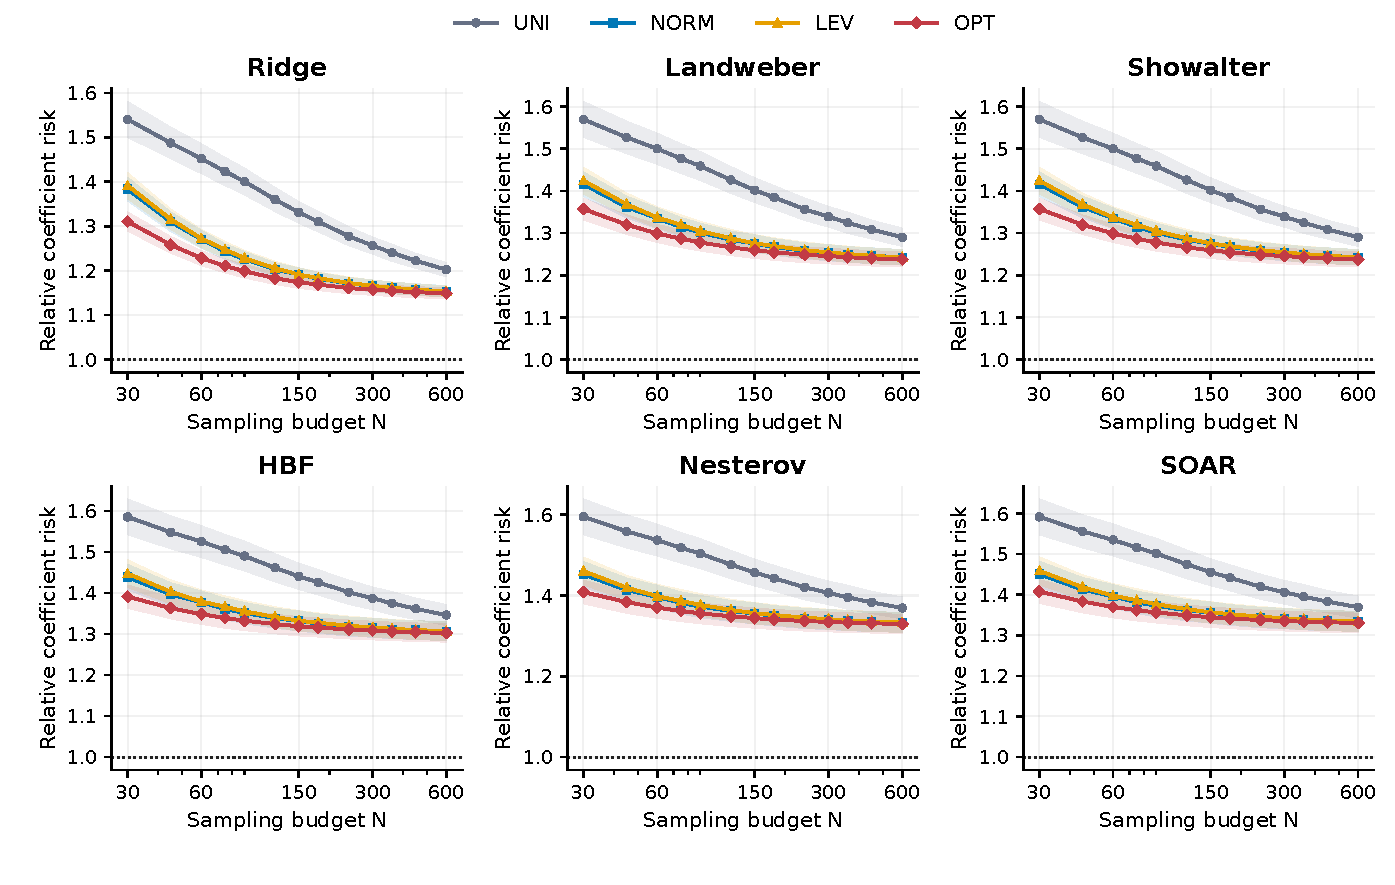
\includegraphics[width=.98\textwidth,trim=0 20bp 0 3bp,clip]{figures/03_true_coefficient_risk.pdf}
\caption{Relative squared error against the generating coefficient, with pointwise intervals across data-set means. The horizontal line is the zero-predictor risk.}
\label{fig:native_coef}
\end{figure}


Eight prespecified one-factor arms use the first six data sets, budgets
$30,90,150,600$, and ten paired sketches: noise levels 0.1/1,
regularization multipliers 0.5/2, uniform-floor masses 0.005/0.05,
homogeneous columns and lognormal heterogeneity parameter 1.5.
Each recalibrates its own targets, influences and OPT, with separate sketch
streams. At $N=150$, all 48 method--arm means favor OPT over NORM;
ratios range from 0.609 to 0.744. These are descriptive sensitivity results.

All 499,200 main, 46,080 robustness and 720 zero-response records are
retained. All main computations have finite outputs; the largest main
relative target error is 1.81.
The boundary checks use two deterministic zero responses, budgets
$30,150,600$, and five sketches; relative errors remain undefined.
Full tails and leave-one-data-set sensitivity envelopes remain in the archive.



\section{Experiment II: row probabilities}
\label{supp:sec:native_exp2}
\subsection{Design and joint row perturbations}
For each of 40 new data sets, draw independent standard Gaussian
$G,K\in\mathbb R^{1200\times60}$ and choose exactly 36 rows uniformly.
With their indicator $m$, set
\[
 R=0.25G+8\operatorname{diag}(m)K,\qquad
 a=\sqrt{60/\|R\|_F^2},\qquad X=aR.
\]
Rescale an independent Gaussian coefficient direction to
$\|X\beta_0\|/\sqrt{1200}=1$ and use $Y=X\beta_0+0.5\xi$.
Data and sampling seeds are 202610240604 and 202610240603, respectively. Budgets and the
40 paired sketches per configuration match Experiment I's grid.

Use $A=X^\top X$, $c=X^\top Y$, $\alpha=\operatorname{tr}(A)/60=1$,
and the shared algorithms. Construct $L$ by Experiment I's complete-data
atom procedure, now using row norms, joint row influences and row
probabilities. The fallback is $1200\max_i\|x_i\|^2/\varepsilon$;
every iterative sketch then satisfies $\|\widehat A\|\leq L$.
Leverage is $x_i^\top A^{-1}x_i$. Both Gram and response use the same
$N_i/(N\pi_i)$ weights. The returned state is already the coefficient;
its tangent includes $-x_ix_i^\top\beta+x_iY_i$.
The fixed-generator local and tail argument is the same as in I, applied
to this coupled numerical estimator.

\subsection{Inference, risks, and sampled-row coverage}
Independent data-set means and pointwise $t_{39}$ intervals are used.
OPT has the smallest mean in 78/78 method--budget cells. The 18
prespecified two-sided paired comparisons at $N=150$ all support lower
OPT error after their own Holm correction (largest reported adjusted
$p<3\times10^{-25}$); all Bonferroni 95\% intervals are below zero.
Table~\ref{tab:row_native_primary} gives the effects; this family
is separate from I's comparisons. At $N=150$, OPT/NORM mean target-MSE
ratios range from 0.305 to 0.394; at $N=600$, they range from 0.208 to 0.321.

\begin{table}[!htbp]
\centering\small
\caption{Native row sampling at the prespecified budget $N=150$. Each entry averages 40 independent data-set means, each based on 40 paired sketches. Ratios compare mean relative target MSE; smaller values favor OPT.}
\label{tab:row_native_primary}
\begin{tabular}{lrrrr}\toprule
Method & OPT MSE & / UNI & / NORM & / LEV \\\midrule
Ridge & 0.05953 & 0.075 & 0.305 & 0.559 \\
Landweber & 0.05747 & 0.073 & 0.339 & 0.554 \\
Showalter & 0.05743 & 0.073 & 0.339 & 0.553 \\
HBF & 0.05881 & 0.074 & 0.371 & 0.553 \\
Nesterov & 0.05884 & 0.074 & 0.388 & 0.543 \\
SOAR & 0.05924 & 0.075 & 0.394 & 0.544 \\
\bottomrule\end{tabular}
\end{table}

For a future row from the 3\% spike mixture, conditional on training
normalization,
\[
 \Sigma=a^2(0.25^2+0.03\times8^2)I.
\]
Consequently population relative signal risk equals coefficient risk
algebraically, giving two expressions of the same risk quantity.
Future-response MSE adds noise variance 0.25. Spike/background signal
risks restrict numerator and denominator to the corresponding row groups.
Table~\ref{tab:row_native_risks} and Figure~\ref{fig:row_native_coef}
retain the distinction between approximation and true risk.
At $N=600$, equal averaging over the six methods gives OPT relative
target MSE 0.01189, coefficient risk 0.501, and in-design signal risk
0.08346; the matching full-target risks are 0.4954 and 0.07795.

\begin{table}[!htbp]
\centering\small
\caption{Separate row risks at $N=600$ for OPT, averaged over 40 data sets. Full coef. is the coefficient risk of the matching full target. Future MSE includes response noise. Population relative signal risk equals Coef. in this isotropic design.}
\label{tab:row_native_risks}
\begin{tabular}{lrrrrr}\toprule
Method & Target gap & Coef. & Full coef. & Design & Future MSE \\\midrule
Ridge & 0.01189 & 0.5424 & 0.5369 & 0.1423 & 0.8237 \\
Landweber & 0.01128 & 0.4989 & 0.4931 & 0.07345 & 0.779 \\
Showalter & 0.01129 & 0.499 & 0.4931 & 0.07347 & 0.779 \\
HBF & 0.01208 & 0.4869 & 0.4811 & 0.06153 & 0.7663 \\
Nesterov & 0.01236 & 0.489 & 0.4834 & 0.0737 & 0.7679 \\
SOAR & 0.01242 & 0.49 & 0.4846 & 0.07635 & 0.7688 \\
\bottomrule\end{tabular}
\end{table}

\begin{figure}[!htbp]\centering
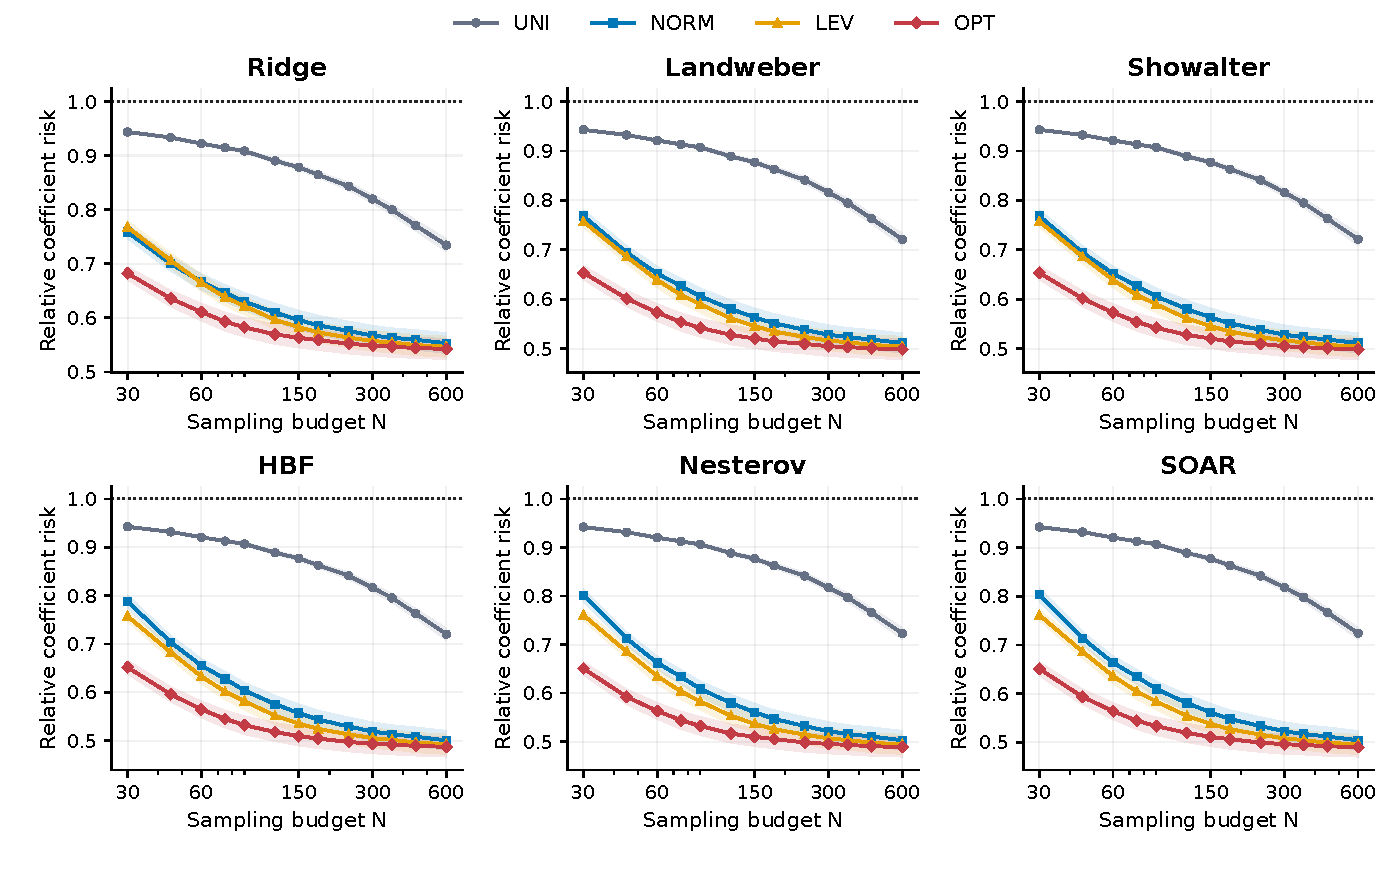
\includegraphics[width=.98\textwidth,trim=0 20bp 0 3bp,clip]{figures/r2_03_true_coefficient_risk.pdf}
\caption{Relative true coefficient risk for native row sampling. The dotted unit reference is the zero predictor; population relative signal risk is identical for this isotropic future-row mixture.}
\label{fig:row_native_coef}
\end{figure}


At $N=30$, UNI draws no designated spike in 38.0\% of sketches; OPT's
observed fraction is zero. Mean distinct-row counts are 29.67 for UNI and
22.86--24.05 for OPT. Such low-coverage and repeated-row draws remain included.
The eight robustness arms use I's replication grid, replacing its two
heterogeneity arms by no added spikes and spike standard deviation 12.
Each arm rescales its own design and coefficient direction and recomputes
targets and influences. At $N=150$, all 48 method--arm means favor OPT
over NORM, with ratios 0.217--0.770. These are descriptive sensitivity results.

All 499,200 main, 46,080 robustness and 720 zero-response records are
retained. All main computations have finite outputs; the largest main
relative target error is 5.52. Boundary checks
use two zero responses, three budgets and five sketches as in I.
The archive retains all tails, spike/background risks and leave-one-data-set
sensitivity results.



\section{Experiment III: first-order MSE calibration}
\label{supp:sec:native_exp3}
\subsection{Design and fixed numerical targets}
Use 20 fresh data sets in each direction from I--II's models, with noise
standard deviation 0.5. Data and sampling seeds are 202610240704 and
202610240703, respectively.
The first predesignated data set per direction uses budgets
\[
 30,60,90,150,240,360,600,1200,2400,4800,9600,19200,38400
\]
and 500 sketches per budget; the other 19 use $N=1200,19200$ with 500
sketches. All six methods share exact uniform multinomial counts over
1200 atoms, giving 306,000 main records. Counts repeat atoms and may
miss spikes or contain fewer than 60 distinct atoms; all such draws remain.

Use the shared algorithms with $\alpha=\operatorname{tr}(M)/60$ and
$L=1200\max_i\|z_i\|^2$. This UNI-specific support bound changes the
calibration from I--II; full targets and tangents are recomputed before
sampling. Both Gram and response are weighted in rows.

\subsection{Unfitted constant and error decomposition}
Using the coefficient influences $J_i$ of
Section~\ref{supp:sec:native_common}, define $N_0 =1200$,
$\bar J=N_0 ^{-1}\sum_iJ_i$, and
\[
 C_m=\frac{N_0 \sum_i\|J_i-\bar J\|^2}{\|\beta_m\|^2},\qquad
 Z=\sum_iJ_i(N_0 N_i/N-1),\qquad
 R=(\widehat\beta_m-\beta_m)-Z.
\]
Equivalently, let $b_m$ be the complete numerical state and $V_i$
its atom influence, with $\bar V=N_0^{-1}\sum_iV_i$.
Then
\[
 C_m=\frac{N_0\sum_i\|V_i-\bar V\|_Q^2}{\|b_m\|_Q^2},
 \qquad Q=\begin{cases}XX^\top,&\text{columns},\\I,&\text{rows}.\end{cases}
\]
Thus coefficient coordinates give the same norms as $XX^\top$-weighted
dual states in columns and ordinary state norms in rows. $C_m$ is computed
before sketches, not fitted. Each actual draw satisfies
\[
 \|\widehat\beta_m-\beta_m\|^2=\|Z\|^2+\|R\|^2+2Z^\top R.
\]
Tables~\ref{tab:v7_robustness}--\ref{tab:v7_decomposition} and
Figure~\ref{fig:v7_mse_ratio} retain finite-budget deviations and signed
cross terms. Near-one total MSE ratios do not by themselves make the
remainder negligible. Intervals use pointwise conditional $t_{499}$;
between-data-set ranges are observed variation, not confidence intervals.

\begin{table}[!htbp]\centering\small
\caption{Empirical-to-theoretical MSE ratios at $N=19200$ across 20 fresh data sets per direction, each with 500 sketches. Ranges are observed variation, not confidence intervals.}
\label{tab:v7_robustness}
\begin{tabular}{llrr}\toprule
Direction & Method & Median & Minimum--maximum \\\midrule
Column & Ridge & 1.012 & [0.9906, 1.031] \\
Column & Landweber & 0.9972 & [0.9755, 1.021] \\
Column & Showalter & 0.9972 & [0.9755, 1.021] \\
Column & HBF & 0.9942 & [0.9683, 1.021] \\
Column & Nesterov & 0.9945 & [0.9677, 1.022] \\
Column & SOAR & 0.9948 & [0.9669, 1.023] \\
Row & Ridge & 1.105 & [1.063, 1.125] \\
Row & Landweber & 1.118 & [1.064, 1.139] \\
Row & Showalter & 1.118 & [1.064, 1.139] \\
Row & HBF & 1.117 & [1.054, 1.149] \\
Row & Nesterov & 1.106 & [1.041, 1.133] \\
Row & SOAR & 1.103 & [1.039, 1.129] \\
\bottomrule\end{tabular}
\end{table}

\begin{figure}[!htbp]\centering
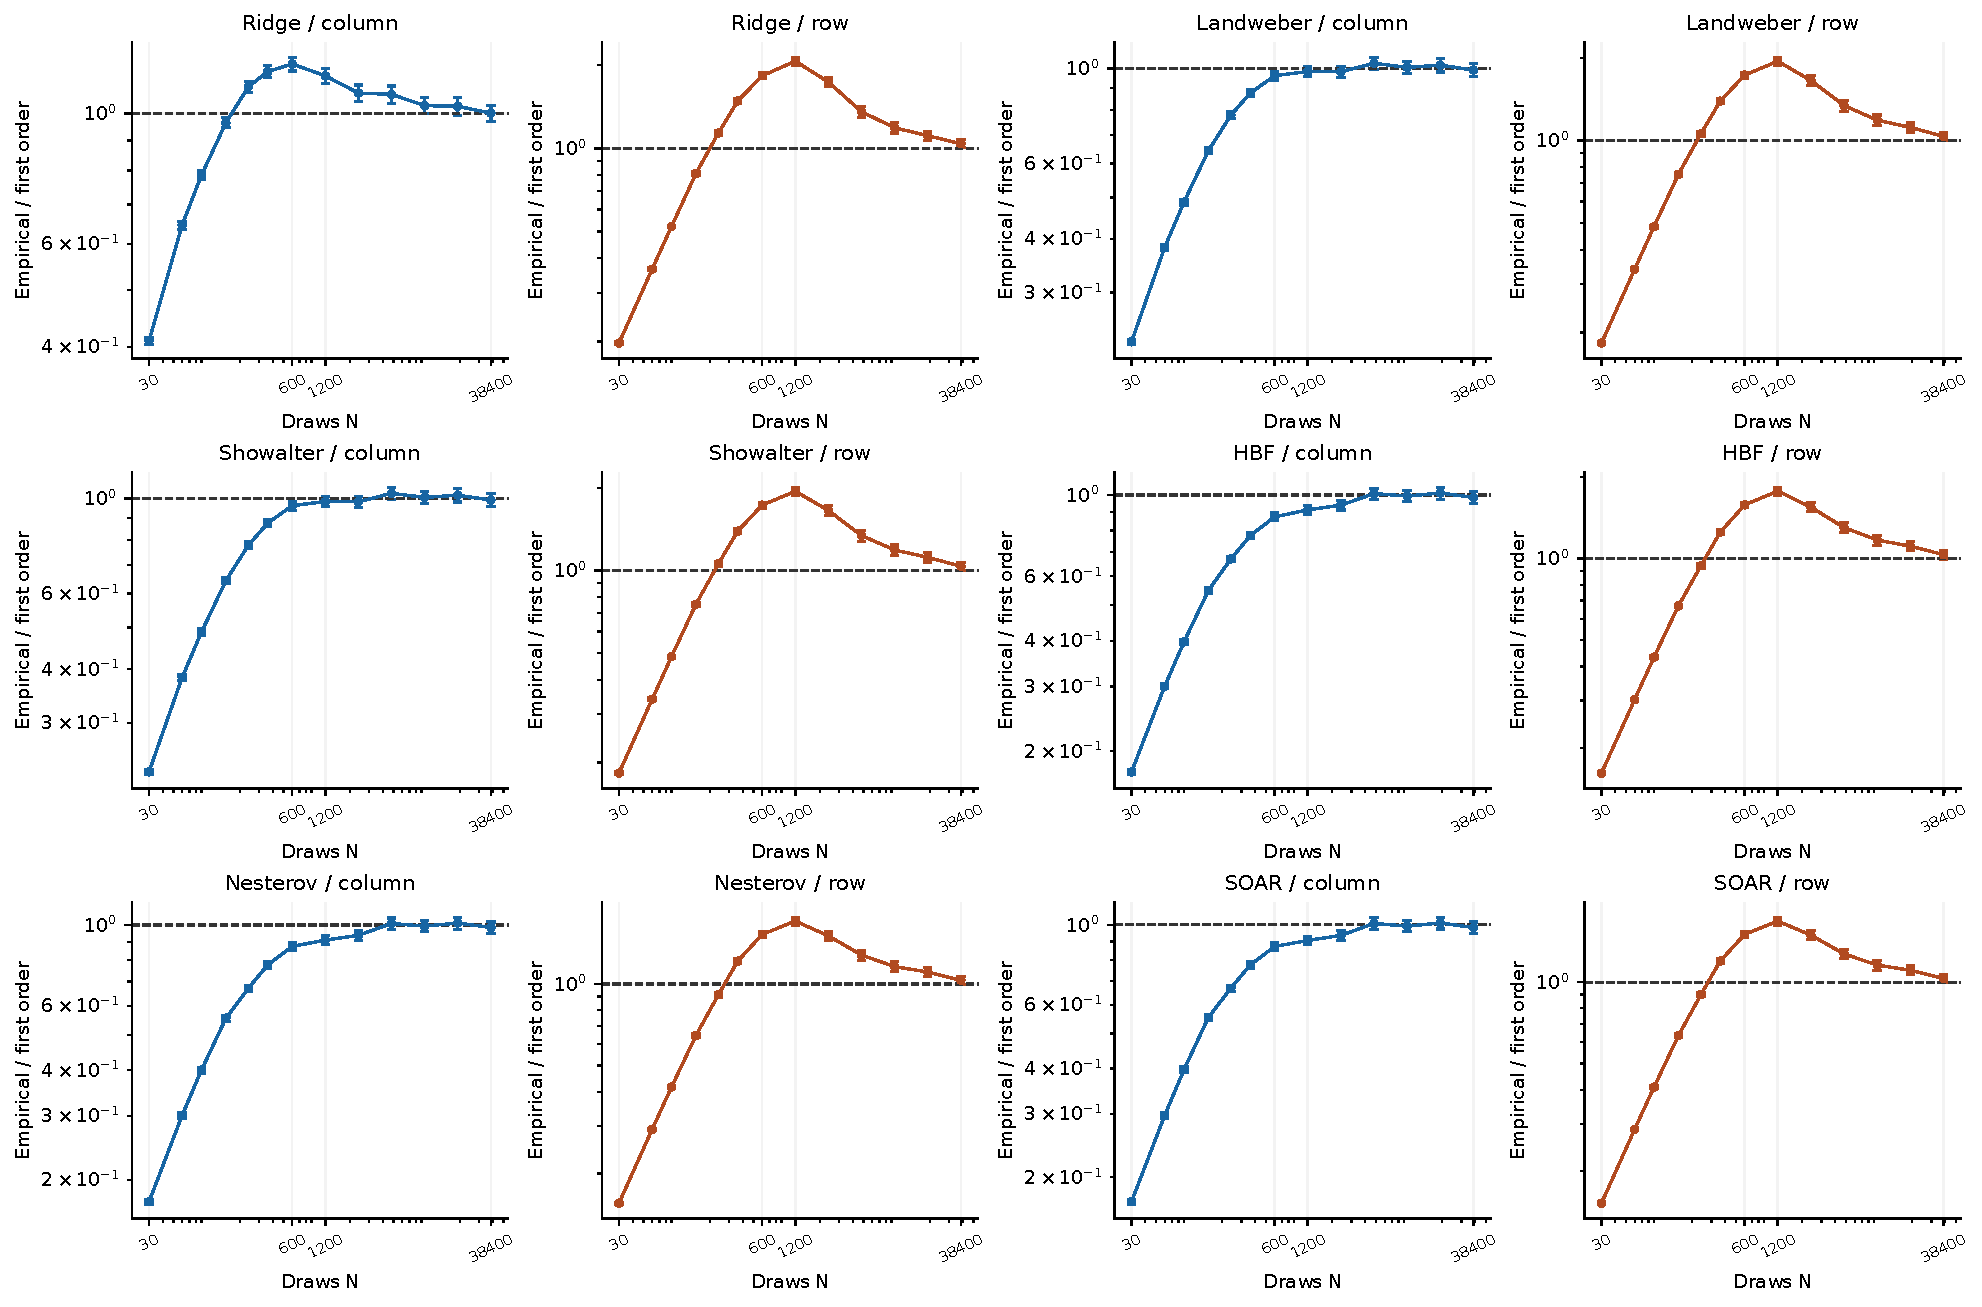
\includegraphics[width=.98\textwidth]{figures/r3_02_mse_ratio.pdf}
\caption{Empirical-to-first-order MSE ratios on the first data set per direction; 500 sketches and pointwise 95\% Monte Carlo intervals. Both axes are logarithmic.}
\label{fig:v7_mse_ratio}
\end{figure}

\begin{table}[!htbp]\centering\small
\caption{Native error decomposition at $N=38400$ on the first data set per direction. Every component is normalized by $C_g/N$; signed cross terms are retained.}
\label{tab:v7_decomposition}
\begin{tabular}{llrrrr}\toprule
Direction & Method & Total & Linear & Remainder & Cross \\\midrule
Column & Ridge & 1.002 & 0.9912 & 0.006494 & 0.003961 \\
Column & Landweber & 0.9909 & 0.9872 & 0.003817 & -0.0001188 \\
Column & Showalter & 0.9909 & 0.9872 & 0.00382 & -0.000114 \\
Column & HBF & 0.9845 & 0.9844 & 0.001734 & -0.001635 \\
Column & Nesterov & 0.9841 & 0.9841 & 0.001483 & -0.001556 \\
Column & SOAR & 0.9836 & 0.9839 & 0.001295 & -0.001581 \\
Row & Ridge & 1.039 & 0.9935 & 0.02636 & 0.01876 \\
Row & Landweber & 1.038 & 0.9876 & 0.03558 & 0.01502 \\
Row & Showalter & 1.038 & 0.9876 & 0.03556 & 0.01502 \\
Row & HBF & 1.034 & 0.9847 & 0.05116 & -0.002159 \\
Row & Nesterov & 1.032 & 0.985 & 0.04977 & -0.002753 \\
Row & SOAR & 1.032 & 0.9851 & 0.0504 & -0.00393 \\
\bottomrule\end{tabular}
\end{table}


\subsection{Sensitivity and scope}
Scale arms use $\alpha=c\operatorname{tr}(M)/60$, $c=0.5,2$, on the
first two data sets per direction, at $N=1200,19200$ with 100 sketches:
9,600 records. Each recomputes parameters, targets and tangents with a
separate sketch stream; these checks are descriptive. Zero-response
checks use two data sets per direction, three budgets and five sketches:
360 records with undefined relative errors and calibration ratios.
All 315,960 records remain, including the maximum main relative target
error 1.364 and all remainder/cross terms.

At $N=38400$ on the first data set, true coefficient risks range from
1.189 to 1.399 for columns and 0.4486 to 0.5038 for rows. Population,
in-design and response risks are archived separately; the row population
signal and coefficient risks coincide algebraically. Budgets exceeding
1200 explore the fixed-data limit.



\section{Experiment IV: changing paths and same-draw LS}
\label{supp:sec:native_exp4}
\label{supp:sec:v7_numerics}
\subsection{Fresh data and frozen parameter paths}
\label{supp:subsec:simulation_settings}
Use five fresh data sets per direction from I--II's models. Data and sampling
seeds are 202610250804 and 202610250803, respectively. The first predesignated data set
uses 100 uniform sketches at each of III's 13 budgets; the other four
use 30 at $N=1200,19200$. The six methods share each count vector and
its LS reference, giving 18,480 records. Independent 1000-sketch arms
at $N=60$ for HBF, Nesterov and SOAR add 6,000 records; zero-response
arms at $N=30,1200$ add 72.

\label{supp:subsec:ls_paths}
For the complete Gram $M$, 48 Cholesky positive-definiteness bisections
bracket its smallest eigenvalue without an eigendecomposition. With accepted
lower endpoint $\ell$, use
\[
 a=\ell/2,\quad b=\|M\|_\infty+a,\quad
 L=\max\{b,1200\max_i\|z_i\|^2\},\quad h=0.9/L.
\]
Here $L$ bounds every uniform sketch. The complete-data and budget-based paths are
\begin{align*}
 \text{Ridge: }&\alpha_N=a/(N-1),\\
 \text{Landweber: }&k_N=\lceil\log N/[-\log(1-ha)]\rceil,\\
 \text{Showalter: }&T_N=\log(N)/a,\\
 \text{HBF: }&\eta=2\sqrt a,\quad T_N=u_N/\sqrt a,
              \quad(1+u_N)e^{-u_N}=1/N,\\
 \text{Nesterov: }&\omega=1,\quad
 k_N=\max\{1,\lceil2\log N/[-\log(1-ha)]-1\rceil\},\\
 \text{SOAR: }&s=1/2,\quad T_N=N/\sqrt a.
\end{align*}
Use the shared native recurrences and maximum RK4 steps, with each integer
grid rescaled to reach its $T_N$. The paths use the exact-flow residual
envelopes associated with Theorem~\ref{main-thm:ls_equivalence}; the archived
\texttt{residual\_bound} field (design value $1/N$) and its flow-formula checks describe this
design reference, not a certified RK4 bound. For example, with
$R_4(z)=1+z+z^2/2+z^3/6+z^4/24$, Showalter's actual $q_N$-step residual is
\[
 q^{\rm RK4}_N(\lambda)=R_4(-\delta_N\lambda)^{q_N},\qquad
 \delta_N=T_N/q_N.
\]
Taylor's remainder gives $R_4(-x)>e^{-x}$ for $x>0$, hence
$q^{\rm RK4}_N(a)>e^{-aT_N}=1/N$. The finite-grid residual therefore
requires its own bound. Proposition~\ref{prop:iv_rk4_bridge} below
verifies (A4)--(A5), including $\sqrt N\,\rho_N\to0$, for these finite-grid
maps in exact arithmetic under explicit spectral bounds, using a localized window.
Householder orthogonal tridiagonal coordinates reduce each matrix-vector
cost while executing every update in float64 without fastmath.
At $N=38400$, SOAR executes 13,858,604 steps for the first column data set
and 89,323,659 for rows; complete work counts are archived.

\subsection{Exact-arithmetic verification of the finite-grid RK4 paths}
\label{supp:subsec:rk4_bridge}

The finite-grid numerical map is the estimator considered here.
Write $g_{m,N}^{\rm num}(\lambda)$ for the
scalar output with unit forcing and zero initial state, and put
$\mathfrak{r}_{m,N}(\lambda)=1-\lambda g_{m,N}^{\rm num}(\lambda)$.
The following result uses the localized-window option in
Assumption~\ref{main-ass:residual_window}. All arithmetic in the statement
and proof is exact; floating-point errors are addressed separately below.

\begin{proposition}[RK4 paths satisfying (A4)--(A5)]
\label{prop:iv_rk4_bridge}
Fix $X\ne0$, arbitrary $Y$, and strictly positive sampling probabilities on a
finite atom population. Let $m=\lambda_{\min}^+(XX^\top)$ and
$M_{\max}=\|XX^\top\|_2$. Suppose the frozen constants satisfy
\begin{equation}\label{eq:iv_rk4_spectral_setup}
 0<a<m,\qquad M_{\max}<b\le L,\qquad
 \max_i\frac{\|z_i\|^2}{\pi_i}\le 2L.
\end{equation}
For integer $N\ge2$, use the Showalter, HBF and transformed SOAR paths
specified in Section~\ref{supp:subsec:ls_paths}, with
$\eta=2\sqrt a$ for HBF and $s=1/2$ for SOAR. For each method choose
$q_N=\lceil T_N/\Delta_{\max}\rceil$, $\Delta_N=T_N/q_N$, with
\[
 \Delta_{\max}=\begin{cases}
  0.9/L,&\text{Showalter},\\
  0.2/\max\{\sqrt L,\eta\},&\text{HBF},\\
  0.2/\sqrt L,&\text{SOAR}.
 \end{cases}
\]
Choose any fixed
\[
 0<\delta<\min\{m/2,m-a,b-M_{\max}\},\qquad
 \mathcal W=I_\delta\subset[a,b].
\]
Then these numerical generators satisfy (A4) with
$\sqrt N\,\rho_N\to0$ and satisfy (A5), in both sampling directions.
More specifically, with $c_*=2-e^{2/5}>1/2$ and $u_N$ defined by
$(1+u_N)e^{-u_N}=1/N$, their residuals obey
\begin{equation}\label{eq:iv_rk4_rates}
 \rho_N\le
 \begin{cases}
 N^{-13/20},&\text{Showalter},\\
 C(1+u_N)^{1-c_*}N^{-c_*},&\text{HBF},\\
 N^{-1},&\text{SOAR},
 \end{cases}
\end{equation}
where $C$ is independent of $N$. At every attainable sample eigenvalue,
including zero, an envelope $K_N$ may be chosen of orders $O(N)$,
$O(N(1+\log N))$, and $O(N^2)$, respectively. Thus
Theorem~\ref{main-thm:ls_equivalence} gives the LS-centered limit and its
first-order conditional moment expansions for these exact-arithmetic maps.
The weaker bounds in \eqref{eq:iv_rk4_rates} do not by themselves establish
the theorem's stronger $O(N^{-1})$ bias conclusion for Showalter or HBF.
\end{proposition}

\begin{proof}
The spectral bounds put $I_\delta$ inside $[a,b]$ and every attainable
sample spectrum inside $[0,2L]$. Let
\[
 P(z)=1+z+z^2/2+z^3/6+z^4/24.
\]
RK4 applied to a homogeneous constant-coefficient system with matrix $B$
has one-step matrix $P(\Delta_N B)$. Translating by an equilibrium, or
augmenting an affine forcing by time and a constant coordinate, gives
the identities used below. These identities analyze the prescribed
updates; they do not replace the experimental trajectories.

\medskip\noindent\textbf{Showalter.}
For $\lambda>0$,
\[
 \mathfrak{r}_{{\rm Showalter},N}(\lambda)
   =P(-\Delta_N\lambda)^{q_N}.
\]
Taylor's remainder gives $P(-x)>e^{-x}>0$ for $x>0$. On $[0,0.9]$,
the increasing polynomial $x/2-x^2/6+x^3/24$ is at most
$0.345375<7/20$. Consequently
\[
 0<P(-x)\le1-\tfrac{13}{20}x
               \le e^{-13x/20}.
\]
Since $\lambda\ge a$ on $\mathcal W$ and $T_N=\log(N)/a$, this proves
the first rate in \eqref{eq:iv_rk4_rates}. For the full support,
$\Delta_N\lambda\le1.8<2$. On $[0,2]$, Taylor's remainder gives
$P(-x)>0$, and
\[
 1-P(-x)=x\{1-x/2+x^2(4-x)/24\}\ge0.
\]
Thus the residual lies in $[0,1]$ on $(0,2L]$, and
$|g_{{\rm Showalter},N}^{\rm num}(\lambda)|\le1/\lambda$.
At zero, RK4 integrates $u'=1$ exactly and the natural gain is $T_N$.

\medskip\noindent\textbf{HBF and the critical root.}
Put $A=\sqrt a$ and
\[
 B_\lambda=\begin{pmatrix}0&1\\-\lambda&-2A\end{pmatrix},\qquad
 F_N(z)=P(\Delta_N z)^{q_N}.
\]
For $\lambda>0$ the equilibrium translation gives
\begin{equation}\label{eq:iv_rk4_hbf_identity}
 \mathfrak{r}_{{\rm HBF},N}(\lambda)=e_1^\top F_N(B_\lambda)e_1.
\end{equation}
For $|z|\le1/5$, set $E=e^{1/5}-1$. The Taylor coefficients imply
$|P(z)-1|\le E$ and $|P'(z)-1|\le E$, hence
\[
 \operatorname{Re}\{P'(z)\overline{P(z)}\}
 \ge1-2E-E^2=c_*.
\]
Also $|P(iy)|^2=1-y^6/72+y^8/576\le1$ for $|y|\le1/5$.
Integrating the derivative of $|P(-x+iy)|^2$ along a horizontal segment
in the disk gives
\begin{equation}\label{eq:iv_rk4_left_disk}
 |P(-x+iy)|^2\le1-2c_*x\le e^{-2c_*x}
 \quad(x\ge0,\ x^2+y^2\le1/25).
\end{equation}

For $a\le\lambda\le L$, the roots of $B_\lambda$ are
$\mu_\pm=-A\pm i\sqrt{\lambda-a}$ and
$|\Delta_N\mu_\pm|\le1/5$. Define the divided difference
\[
 D_N=\frac{F_N(\mu_+)-F_N(\mu_-)}{\mu_+-\mu_-},
 \quad D_N=F_N'(-A)\quad(\lambda=a).
\]
Polynomial functional calculus, including the repeated-root limit, yields
\[
 \mathfrak{r}_{{\rm HBF},N}(\lambda)
 =\frac{F_N(\mu_+)+F_N(\mu_-)}2+A D_N.
\]
The segment joining the roots lies on $\operatorname{Re}z=-A$ and
stays in the same scaled disk. By \eqref{eq:iv_rk4_left_disk},
$|P'(\Delta_N z)|\le e^{1/5}$ there, and $A\Delta_N\le1/10$,
\[
 |D_N|\le\sup_{z\in[\mu_-,\mu_+]}|F_N'(z)|
 \le e^{2/5}T_N e^{-c_*AT_N}.
\]
This proves $\rho_N\le e^{2/5}(1+u_N)e^{-c_*u_N}$, including
$\lambda=a$. Substituting $e^{-u_N}=1/[N(1+u_N)]$ gives the HBF rate.
Moreover $u_N=O(\log N)$, so $\sqrt N\,\rho_N\to0$.

For the full interval $0\le\lambda<a$, both roots are real in $[-2A,0]$;
their scaled segment lies in $[-1/5,0]$, where $0<P\le1$.
For $a\le\lambda\le2L$, the scaled complex segment has modulus at most
$\sqrt2/5<3/10$. Repeating the disk argument with radius $3/10$ gives
the positive constant $2-e^{3/5}>0$, hence $|P|\le1$ on this segment.
The same divided-difference formula, now using
$|F_N'|\le e^{3/10}T_N$, gives uniformly
\[
 |\mathfrak{r}_{{\rm HBF},N}(\lambda)|
 \le1+e^{3/10}AT_N,\qquad
 |g_{{\rm HBF},N}^{\rm num}(\lambda)|
 \le\frac{2+e^{3/10}AT_N}{\lambda}\quad(\lambda>0).
\]
At zero, the equation $v'=1-\eta v$ and the affine invariant
$(u+v/\eta)'=1/\eta$, both preserved by RK4, give
\begin{equation}\label{eq:iv_rk4_hbf_zero}
 g_{{\rm HBF},N}^{\rm num}(0)
 =\frac{T_N}{\eta}
  -\frac{1-P(-\eta\Delta_N)^{q_N}}{\eta^2}.
\end{equation}
Its absolute value is at most $T_N/\eta+1/\eta^2$.

\medskip\noindent\textbf{Transformed SOAR.}
For $\lambda>0$, set
$C_\lambda=\left(\begin{smallmatrix}0&1\\-\lambda&0\end{smallmatrix}\right)$.
The particular state $(t/\lambda,1/\lambda)^\top$ of
$w''+\lambda w=t$ is preserved exactly by the RK4 stages.
Subtracting it from the zero initial state gives
\begin{equation}\label{eq:iv_rk4_soar_identity}
 \mathfrak{r}_{{\rm SOAR},N}(\lambda)
 =\frac{e_1^\top P(\Delta_N C_\lambda)^{q_N}e_2}{T_N}
 =\frac{\operatorname{Im}\{P(i\Delta_N\sqrt\lambda)^{q_N}\}}
        {T_N\sqrt\lambda}.
\end{equation}
On $[0,2L]$, $\Delta_N\sqrt\lambda\le\sqrt2/5<\sqrt8$.
The imaginary-axis identity gives $|P(iy)|\le1$ for $|y|\le\sqrt8$,
and therefore $|\mathfrak{r}_{{\rm SOAR},N}(\lambda)|
\le1/(T_N\sqrt\lambda)$. On $\mathcal W$, $T_N=N/\sqrt a$ therefore
gives $\rho_N\le1/N$. On all positive sample eigenvalues,
\[
 |g_{{\rm SOAR},N}^{\rm num}(\lambda)|
 \le\lambda^{-1}+(T_N\lambda^{3/2})^{-1}.
\]
At zero, RK4 integrates the cubic solution $w(t)=t^3/6$ exactly,
so $g_{{\rm SOAR},N}^{\rm num}(0)=T_N^2/6$.

\medskip\noindent\textbf{Tail control and conclusion.}
Lemma~\ref{lem:finite_atoms} gives a fixed $\kappa>0$, independent of $N$, such that every
attainable positive sample eigenvalue is at least $\kappa/N$.
The positive-spectrum and zero-spectrum bounds just proved give
$K_N\le CN$, $CN(1+\log N)$ and $CN^2$, respectively, after enlarging
$C$ to cover all $N\ge2$. Thus $\log K_N=O(\log N)=o(N)$, and
Proposition~\ref{main-prop:tail_envelope} verifies (A5) with the same
fixed good-event radius $\delta$. All three rates verify the root-$N$
part of (A4). The claimed conclusions follow from
Theorem~\ref{main-thm:ls_equivalence}.
\end{proof}

\begin{remark}[Scope of the numerical verification]
\label{rem:iv_rk4_scope}
Condition~\eqref{eq:iv_rk4_spectral_setup} requires a strict lower
window margin $a<m$, not the stronger $a\le m/2$ or an exact identification
of a Cholesky bisection endpoint. The local window $I_\delta$, rather
than the default $[m/2,M_{\max}+m/2]$, is essential to this formulation.
For uniform sampling, the ideal definition
$L\ge1200\max_i\|z_i\|^2$ supplies the stronger support bound $B\le L$;
the factor-two allowance in \eqref{eq:iv_rk4_spectral_setup} also avoids
requiring an exactly upward-rounded stored value of $L$.
For all ten IV input data sets, exact-integer congruence and row-sum
checks on the saved binary inputs verify
\eqref{eq:iv_rk4_spectral_setup} with the stored $a,b,L$.
These checks establish the spectral inequalities for the saved binary inputs.
The proposition concerns the real-arithmetic algorithm with the stated
parameter paths. The numerical results below use float64 arithmetic and
tolerance-based QR ranks, with selected replay and grid diagnostics.
\end{remark}


\subsection{QR reference, observed gaps, and numerical resolution}
\label{supp:subsec:ls_numerics}
Let $Z$ have nonzero columns $z_i\sqrt{1200N_i/N}$, so $M_N=ZZ^\top$.
The column reference is $X^\top M_N^\dagger Y$, obtained from two
minimum-norm solves on $Z$ and $Z^\top$. Rows solve the jointly weighted
design/response problem. Both use LAPACK GELSY with pivoted QR and relative
threshold $10^{-12}$. An independent column-space QR construction checks
the references. Rank-deficient sketches and null-response components remain.
Iterative outputs and LS references are compared as distinct coefficient vectors.

The actual coefficient vectors are subtracted to form
$D_m(N)=N\,\operatorname{mean}\|\widehat\beta_{m,N}-\widehat\beta_{\rm LS}\|^2$.
All 12 direction--method endpoint means decrease from 1200 to 38400
(Table~\ref{tab:exp4_endpoints}). Pointwise intervals use $t_{99}$ on the
first data set and $t_{29}$ on the other four.

\begin{table}[!htbp]\centering\small
\caption{Untrimmed mean scaled squared gap $D(N)$, on the first new data set per direction. A dagger marks resolution-limited high-budget Nesterov values and their derived ratios: selected replay changes exceed the observed gaps.}
\label{tab:exp4_endpoints}
\begin{tabular}{llrrr}\toprule
Direction & Method & $D(1200)$ & $D(38400)$ & Ratio \\\midrule
Column & Ridge & 0.0003744 & 2.93e-06 & 0.007826 \\
Column & Landweber & 1.865e-06 & 3.369e-15 & 1.806e-09 \\
Column & Showalter & 1.867e-06 & 3.381e-15 & 1.811e-09 \\
Column & HBF & 1.568e-05 & 1.27e-07 & 0.0081 \\
Column & Nesterov & 8.063e-13 & 4.961e-22$^{\dagger}$ & 6.153e-10$^{\dagger}$ \\
Column & SOAR & 0.0003815 & 4.225e-06 & 0.01107 \\
Row & Ridge & 0.2291 & 0.003352 & 0.01463 \\
Row & Landweber & 2.943e-05 & 9.967e-13 & 3.386e-08 \\
Row & Showalter & 2.944e-05 & 9.968e-13 & 3.387e-08 \\
Row & HBF & 0.01221 & 0.0001243 & 0.01018 \\
Row & Nesterov & 3.459e-13 & 2.017e-15$^{\dagger}$ & 0.005832$^{\dagger}$ \\
Row & SOAR & 0.2715 & 0.004434 & 0.01633 \\
\bottomrule\end{tabular}
\end{table}


The arithmetic scale
$64\epsilon_{\rm mach}\max\{1,\|\widehat\beta\|,\|\widehat\beta_{\rm LS}\|\}$
flags close-vector subtraction without bounding accumulated iteration error.
Table~\ref{tab:exp4_replay} compares independent native replays with the
observed gaps. Nesterov replay discrepancies are 1.385 and 1.071 times
the two high-budget gaps, so those tiny gaps do not resolve superior
attainable accuracy. Twelve doubled-grid checks are also archived;
their largest change/gap ratio is 0.01764, for row Showalter at 38400.

\begin{table}[!htbp]\centering\small
\caption{Independent dense-coordinate replay at $N=38400$, rep=0. Relative coefficient discrepancy is normalized by max(1, LS norm); the last column compares that discrepancy with the observed gap. This is a diagnostic for the selected configuration.}
\label{tab:exp4_replay}
\begin{tabular}{llrr}\toprule
Direction & Method & Relative change & Change/gap \\\midrule
Column & Ridge & 7.733e-16 & 9.265e-11 \\
Column & Landweber & 4.622e-14 & 0.0001617 \\
Column & Showalter & 4.595e-14 & 0.0001605 \\
Column & HBF & 1.786e-15 & 9.422e-10 \\
Column & Nesterov & 1.422e-13 & 1.385$^{\dagger}$ \\
Row & Ridge & 1.049e-14 & 1.369e-09 \\
Row & Landweber & 1.7e-12 & 0.01018 \\
Row & Showalter & 1.701e-12 & 0.01019 \\
Row & HBF & 2.24e-14 & 1.411e-08 \\
Row & Nesterov & 6.153e-12 & 1.071$^{\dagger}$ \\
\bottomrule\end{tabular}
\end{table}


The reproducibility release reports the local subtraction floor and selected
independent replay discrepancies in separate fields. The floor describes
close-vector subtraction; replay comparisons assess accumulated numerical
differences in the selected configurations.

\subsection{Low-budget tails and separate true risks}
Table~\ref{tab:exp4_tails} retains the independent low-budget tail arms.
Large differences between means and medians and concentration in the top
1\% limit expectation estimation at this replication. These arms are
summarized separately from the primary means.

\begin{table}[!htbp]\centering\small
\caption{Untrimmed independent $N=60$ tail arms, 1000 sketches each. Values summarize the scaled squared gap; the final column is the fraction of the sum contributed by the highest 1 percent.}
\label{tab:exp4_tails}
\begin{tabular}{llrrrr}\toprule
Direction & Method & Mean & Median & Maximum & Top 1 percent \\\midrule
Column & HBF & 7.227e+17 & 1.467e+09 & 6.949e+20 & 1 \\
Column & Nesterov & 7.227e+17 & 1.302e+11 & 6.949e+20 & 1 \\
Column & SOAR & 7.227e+17 & 1.203e+09 & 6.949e+20 & 1 \\
Row & HBF & 1.897e+09 & 1.931e+07 & 7.109e+11 & 0.8975 \\
Row & Nesterov & 1.105e+09 & 170.9 & 6.872e+11 & 0.9995 \\
Row & SOAR & 1.869e+09 & 8.5e+05 & 7.109e+11 & 0.9105 \\
\bottomrule\end{tabular}
\end{table}


At $N=38400$, all six methods have, to the reported precision, column
coefficient/design/population risks 2.017/19.54/5.226 and future-response
MSE 0.3229; row values are 0.2911/0.01416/0.2911 and 0.494.
All 24,552 records are retained; zero-target relative LS errors remain undefined.



\section{Experiment V: full-size real data}
\label{supp:sec:native_exp5}
\subsection{Data, preprocessing, and changed step protocol}
\label{supp:subsec:real_protocol}
GDSC uses release-6.0 expression file
\path{sanger1018_brainarray_ensemblgene_rma.txt.gz} and release-8.4
\path{GDSC2_fitted_dose_response_24Jul22.csv}, with MG-132
identifier 1862. Retain all 937 matched finite-response cells and 17,737
genes, excluding duplicate expression cell columns.
The historical seed-20261020 identifier split has 749 training and 188
test cells.
YearPredictionMSD uses its official 463,715/51,630 training/test split
and all 90 features. Means, scales and response intercepts are fitted on
training data.

GDSC retains $c=1$ for every method. Year retains historical full-model
validation choices: $c=10^{-6}$ for Ridge, $0.001$ for Landweber,
Showalter and HBF, and $10^{-5}$ for Nesterov and SOAR. Set
$\alpha=c\operatorname{tr}(M)/d_0$, with $d_0=749$ for columns and
$90$ for rows. The single fixed splits and prior test exploration make
prediction results descriptive.

The new protocol changes the step scale to $L=32\|M\|_\infty$ while
retaining those $c$ values and continuous endpoints. Use the shared frozen
count and grid formulas; targets, derivatives and OPT are recomputed and
sealed before sampling. Table~\ref{tab:rd_min_parameters} gives actual
parameters. Householder tridiagonal coordinates execute every recurrence
and RK4 stage in float64. $L$ is not a bound on the entire sampling
support. Each realized matrix receives a separate Cholesky check of
$LI-M_N$ under the frozen protocol. The 12,720 formal computations show
zero step-bound violations and zero numerical failures. These stability
checks apply to the realized matrices.
Separately, with fixed finite update counts and integration grids, the
numerical generators are polynomials. Positive fixed probabilities give a finite
attainable spectral interval $[0,B]$, with
$B=\max_i\|z_i\|^2/\pi_i$, whether or not $B\le L$.
These polynomials satisfy the fixed-generator local assumptions and
Proposition~\ref{main-prop:fixed_tail_growth}; Ridge is bounded by $1/\alpha$.
The resulting moment statement concerns the exact-arithmetic asymptotic limit.

\begin{table}[!htbp]\centering\small
\setlength{\tabcolsep}{4pt}
\caption{Actual frozen native parameters. Step size means recurrence step or RK4 mesh; Ridge zeros are placeholders. Full-precision endpoints and damping are archived.}
\label{tab:rd_min_parameters}
\begin{tabular}{llrrrr}\toprule
Data & Method & $c$ & $\alpha$ & Steps & Step size \\\midrule
gdsc & Ridge & 1 & 17737 & 0 & 0 \\
gdsc & Landweber & 1 & 17737 & 4371 & 1.29e-08 \\
gdsc & Showalter & 1 & 17737 & 4371 & 1.2898e-08 \\
gdsc & HBF & 1 & 17737 & 783 & 2.3941e-05 \\
gdsc & Nesterov & 1 & 17737 & 161 & 1.29e-08 \\
gdsc & SOAR & 1 & 17737 & 769 & 2.3917e-05 \\
year & Ridge & 1e-06 & 0.46371 & 0 & 0 \\
year & Landweber & 0.001 & 463.71 & 741388 & 2.9087e-09 \\
year & Showalter & 0.001 & 463.71 & 741388 & 2.9087e-09 \\
year & HBF & 0.001 & 463.71 & 10197 & 1.137e-05 \\
year & Nesterov & 1e-05 & 4.6371 & 21090 & 2.9087e-09 \\
year & SOAR & 1e-05 & 4.6371 & 100044 & 1.137e-05 \\
\bottomrule\end{tabular}
\end{table}


\subsection{Native influences, paired draws, and calibration}
Checkpointed reverse differentiation uses the actual finite-grid algorithms,
including joint row Gram/response perturbations. For columns a pivoted-QR
factor $C$ with $C^\top C=XX^\top$ computes the equivalent coefficient
norm $\|X^\top\delta u\|=\|C\delta u\|$; rows use $C=I$.
The orthogonal basis is fixed during differentiation. LEV uses pivoted
QR with relative diagonal rank threshold $10^{-10}$; NORM equals UNI
exactly for standardized GDSC genes. All probabilities remain fixed across budgets.

GDSC budgets are $75,187,374,749,1498,2996$, with 30 paired draws;
Year budgets are $500,1000,2000,5000,10000,20000,50000$, with 50.
Fresh seed 202610250906 is separate from historical runs. Repeated atoms
retain their full weights; all sparse counts and numerical states are saved.
Intervals use conditional $t_{29}$ and $t_{49}$ for the fixed data sets.
For the full-data numerical coefficient $\beta_m$ and sampling rule $\pi$,
the relative target MSE is estimated by
\begin{equation}\label{eq:real_relative_mse}
 \widehat E_{m,\pi}(N)=\frac1B\sum_{b=1}^B
 \frac{\|\widetilde\beta_{m,\pi,N}^{(b)}-\beta_m\|^2}{\|\beta_m\|^2},
\end{equation}
where $B$ is the number of paired draws. This is the empirical version of
the common metric in main Section~\ref{main-subsec:v7_setup}.
For Ridge, the UNI/OPT target-MSE values are 0.044687/0.0287 on GDSC
at $N=2996$ and 0.094986/0.033498 on YearPredictionMSD at $N=5000$.
The unfitted first-order constant is
\[
 C_{m,\pi}=Q_m(\pi)/\|\beta_m\|^2,\qquad
 K(N)=\widehat E_{m,\pi}(N)/(C_{m,\pi}/N).
\]
Table~\ref{tab:real_calibration} shows oracle ratios and OPT calibration
at the smallest and largest budgets; finite-budget deviations from one remain.

\begin{table}[!htbp]\centering\small
\setlength{\tabcolsep}{4pt}
\caption{Native full-coefficient first-order constants and calibration. Constant ratios check the oracle objective; empirical/theory ratios describe conditional finite-budget approximation.}
\label{tab:real_calibration}
\begin{tabular}{llrrrr}\toprule
Data & Method & $C_O/C_U$ & $C_O/C_L$ & $K(N_{\min})$ & $K(N_{\max})$ \\\midrule
gdsc & Ridge & 0.5946 & 0.58481 & 2.522 & 1.1846 \\
gdsc & Landweber & 0.60017 & 0.56969 & 1.9703 & 1.084 \\
gdsc & Showalter & 0.60017 & 0.56969 & 1.9747 & 1.076 \\
gdsc & HBF & 0.60615 & 0.56058 & 1.4991 & 1.0716 \\
gdsc & Nesterov & 0.60648 & 0.55643 & 1.5119 & 1.0567 \\
gdsc & SOAR & 0.607 & 0.55563 & 1.5207 & 1.0157 \\
year & Ridge & 0.32723 & 0.41733 & 2.4244 & 0.99175 \\
year & Landweber & 0.32723 & 0.41733 & 2.4381 & 0.99634 \\
year & Showalter & 0.32723 & 0.41733 & 2.4381 & 0.99634 \\
year & HBF & 0.33371 & 0.48425 & 1.6292 & 1.0157 \\
year & Nesterov & 0.32722 & 0.41741 & 2.5468 & 0.97548 \\
year & SOAR & 0.32814 & 0.42014 & 2.3204 & 0.97939 \\
\bottomrule\end{tabular}
\end{table}


\paragraph{Paired comparisons and inference revision.}
\label{supp:subsec:real_inference_revision}
OPT has the smallest mean coefficient-target error in all 78 method--budget
cells. The frozen protocol specified budgets 749 (GDSC) and 5000 (Year)
and the 36 paired comparisons against UNI, NORM and LEV, but did not
specify sidedness. The original code used one-sided tests. Following the
audit, we report two-sided paired $t$ tests recomputed from the same saved
records, with one joint Holm correction: all 36 differences are negative
and significant, with largest adjusted $p\approx2.9821\times10^{-8}$.
The two-sided reporting choice was made during this reanalysis.
The GDSC NORM/UNI duplicate remains in the family; original one-sided
outputs and the frozen protocol are preserved. The source supplement
includes \path{native_exp5/paired_comparisons_two_sided.csv},
\path{native_exp5/inference_revision.json}, and a read-only reanalysis script
requiring the full saved-record archive. These conditional tests remain
approximate under finite-sample tails and do not adjust for historical
parameter or test-set exploration. Their comparison family is separate from I--II.

\subsection{Prediction and interpretation}
\label{supp:subsec:real_prediction}
Test-target MSE measures deviation from a matched native full-model
prediction; response MSE and mean individual RMSE compare with observed
test outcomes. True coefficients are unknown, and mean RMSE is not the
square root of mean MSE. Table~\ref{tab:real_prediction_compact} and
Figure~\ref{fig:real_native_prediction} retain these auxiliary prediction
results. At GDSC Ridge $N=75$, OPT reduces coefficient-target error but
raises mean test RMSE to 1.780 versus UNI 1.6144. This difference
illustrates the distinction between coefficient approximation and prediction.
All tail and coverage summaries, including low-coverage draws, remain archived.

\begin{table}[!htbp]\centering\small
\setlength{\tabcolsep}{4pt}
\caption{Mean individual test RMSE at each dataset's largest budget, with matched native full-model RMSE.}
\label{tab:real_prediction_compact}
\begin{tabular}{llrrrrr}\toprule
Data & Method & Full & UNI & NORM & LEV & OPT \\\midrule
gdsc & Ridge & 0.566 & 0.57669 & 0.57669 & 0.57697 & 0.56985 \\
gdsc & Landweber & 0.56496 & 0.58192 & 0.58192 & 0.58296 & 0.5739 \\
gdsc & Showalter & 0.56496 & 0.58191 & 0.58191 & 0.58295 & 0.5735 \\
gdsc & HBF & 0.56581 & 0.58553 & 0.58553 & 0.58772 & 0.5765 \\
gdsc & Nesterov & 0.56738 & 0.58986 & 0.58986 & 0.59218 & 0.58664 \\
gdsc & SOAR & 0.56758 & 0.5902 & 0.5902 & 0.59259 & 0.58013 \\
year & Ridge & 9.5102 & 9.5201 & 9.519 & 9.5185 & 9.5139 \\
year & Landweber & 9.5102 & 9.5201 & 9.519 & 9.5185 & 9.5139 \\
year & Showalter & 9.5102 & 9.5201 & 9.519 & 9.5185 & 9.5139 \\
year & HBF & 9.5149 & 9.5255 & 9.5236 & 9.5236 & 9.5188 \\
year & Nesterov & 9.5102 & 9.5201 & 9.519 & 9.5185 & 9.5139 \\
year & SOAR & 9.5102 & 9.5201 & 9.519 & 9.5185 & 9.5135 \\
\bottomrule\end{tabular}
\end{table}

\begin{figure}[!htbp]\centering
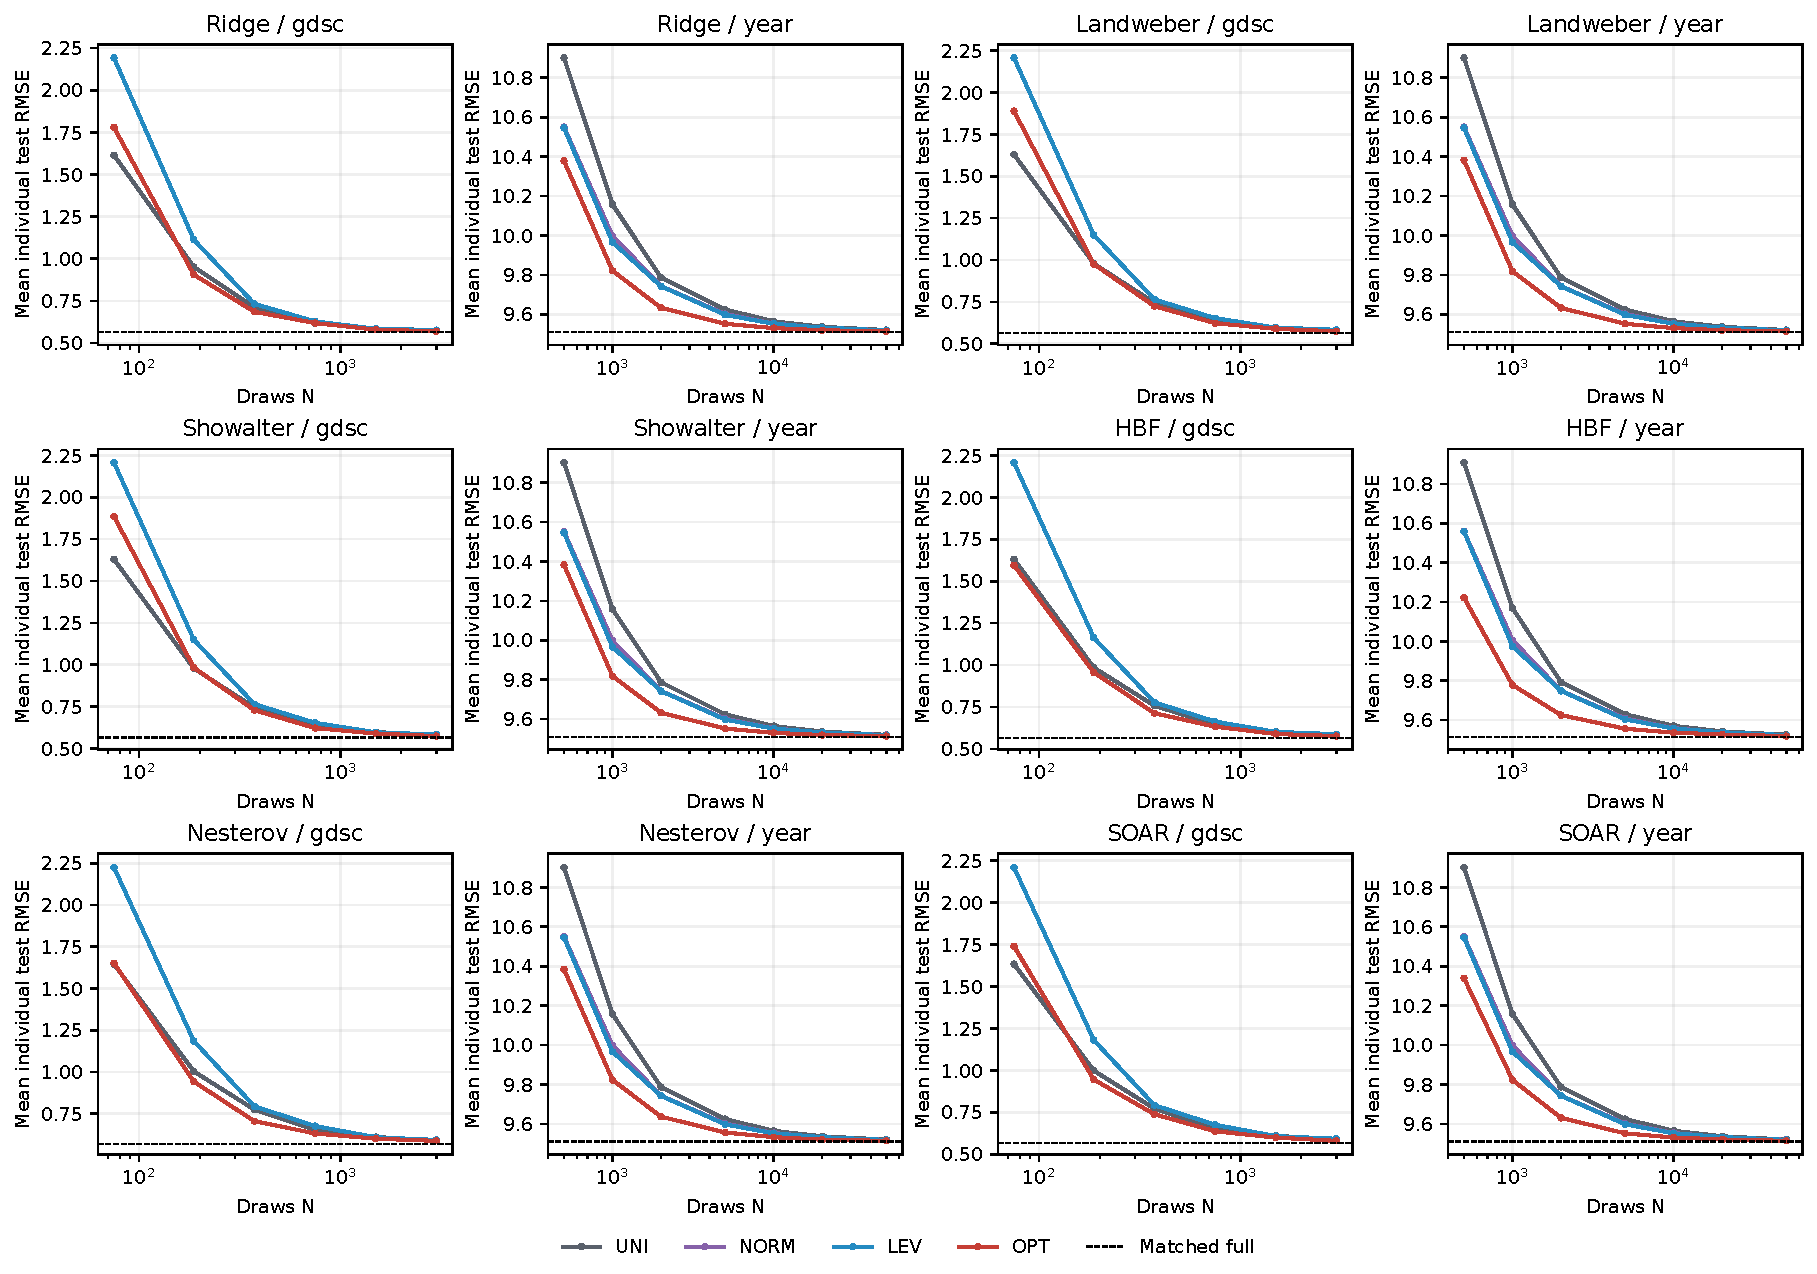
\includegraphics[width=.98\textwidth]{figures/r5_04_prediction.pdf}
\caption{Auxiliary response test RMSE at frozen parameters. Dashed lines are the matched native full-model references. These are descriptive comparisons on previously explored test sets.}
\label{fig:real_native_prediction}
\end{figure}



\subsection{Data and code availability}
\label{supp:subsec:data_code}
The real data are publicly available from the original providers. The GDSC
expression file \path{sanger1018_brainarray_ensemblgene_rma.txt.gz} is available
from the Sanger
\href{https://ftp.sanger.ac.uk/pub/project/cancerrxgene/releases/release-6.0/}{release-6.0 archive}.
The drug-response file \path{GDSC2_fitted_dose_response_24Jul22.csv} is available
from the
\href{https://ftp.sanger.ac.uk/pub/project/cancerrxgene/releases/release-8.4/}{release-8.4 archive}.
YearPredictionMSD, distributed as \path{YearPredictionMSD.txt}, is available
from the \href{https://doi.org/10.24432/C50K61}{UCI Machine Learning Repository,
dataset 203}~\citep{bertin2011year}.
The selected response, preprocessing, and fixed training/test splits are
specified in Section~\ref{supp:subsec:real_protocol}.

The code and associated simulation data are publicly available at
\url{https://github.com/L1wuyang/Subsampling}; the version described here is
\href{https://github.com/L1wuyang/Subsampling/tree/87bc5c50b60c3b71fb89935d2114cef50e7fceb7}{commit \texttt{87bc5c5}}.
The \path{simulations/} directory contains the simulation inputs,
per-repetition metrics, and summary tables for Experiments I--IV.
Its manifest and \path{docs/SIMULATION_DATA.md} document the files and
provide commands for verification and recomputation of the summaries.

The repository includes the source code for Experiments I--V, fixed
protocols and random seeds, the GDSC training/test ID split, dependency
specifications, and provenance records.
The \path{docs/DATA_SOURCES_CN.md} guide and
\path{provenance/data_sources.json} specify the official download URLs,
exact filenames, and checksums of the frozen inputs.
The root \path{run.py} provides commands for data acquisition and
verification, full experimental runs, and analysis of the generated results;
the README documents their use. Simulated inputs can also be regenerated
from the fixed seeds. The Experiment V analysis uses the two-sided
36-comparison Holm family described in
Section~\ref{supp:subsec:real_inference_revision}.

% Independent bibliography for references cited in this supplement.

\begingroup
\renewcommand{\bibfont}{\footnotesize}
\setlength{\bibsep}{2pt plus1pt minus0.5pt}
\FloatBarrier
\bibliographystyle{sn-mathphys-ay}
\bibliography{references}
\endgroup

\end{document}
